\documentclass{article}
\usepackage[top=0.75in, bottom=0.75in, left=1.25in, right=1in]{geometry} %formatage%
\usepackage{amsmath} %pour utiliser des maths de base%
\usepackage{amssymb} %pour faire \mathcal{}=>des lettres ''cursives''%
\usepackage{graphicx} %pour importer des images...http://www.tex.ac.uk/cgi-bin/texfaq2html?label=figurehere%
\usepackage{titlesec} %automatique, pour faire des sous-titres moins laids%
%\usepackage{cancel}
\usepackage[procnames]{listings}
\usepackage[utf8]{inputenc} 
\usepackage[T1]{fontenc}        %http://tex.stackexchange.com/questions/11897/draw-a-diagonal-arrow-across-an-expression-in-a-formula-to-show-that-it-vanishes%
\usepackage[frenchb]{babel}
\usepackage{xcolor}
\usepackage[squaren]{SIunits}
\usepackage{subcaption} % Avoir plusieurs sous-figures (graphiques) dans une figures et pouvoire les étiqueter
\usepackage{color}
\usepackage{lipsum}
\usepackage{caption}
\usepackage{wasysym}
\usepackage{braket}
\usepackage{mathtools}
\usepackage{mathrsfs} % Faire le symbole de la transformée de Laplace
\usepackage{bbm}
\usepackage{array}
\usepackage{diagbox}        
\usepackage{dsfont} % Faire des belles indicatrices                         %diagonale dans les tableaux
\usepackage{float}%placer les tableaux et images où tu veux
\usepackage{listings}
\usepackage[utf8]{inputenc}
\usepackage{comment}
\usepackage{pst-node}
\usepackage{enumitem}
\usepackage{breakcites} % Faire en sorte que les citations ne sortent pas dans la marge
\usepackage{graphicx} % Insérer des graphiques
\usepackage{pgfplots}
\pgfplotsset{width=10cm, compat=1.9}
\usetikzlibrary{patterns,decorations.pathreplacing}

\newcommand{\tikzmark}[2]{%
	\tikz[remember picture,baseline=(#1.base)]
	\node[circle,red,draw,text=black,anchor=center,inner sep=1pt] (#1) {#2};}
\newcommand{\tikzmarkk}[2]{%
	\tikz[remember picture,baseline=(#1.base)]
	\node (#1) {#2};}


%\setcounter{secnumdepth}{0} % sections are level 1

\newtheorem{lemme}{Lemme}
\newtheorem{preuve}{Preuve}
\newtheorem{defini}{Définition}
\newtheorem{propo}{Proposition}
\newtheorem{algo}{Algorithme}
\newtheorem{Scenario}{Scénario}

\begin{document}
	\renewcommand{\figurename}{Illustration}
	\renewcommand{\tablename}{Tableau}
	
		\begin{titlepage}
		\centering % Centre everything on the title page
		
		\scshape % Use small caps for all text on the title page
		
		\vspace*{7\baselineskip} % White space at the top of the page
		
		%------------------------------------------------
		%	Title
		%------------------------------------------------
		
		\rule{\textwidth}{1.6pt}\vspace*{-\baselineskip}\vspace*{2pt} % Thick horizontal rule
		\rule{\textwidth}{0.4pt} % Thin horizontal rule
		
		\vspace{0.75\baselineskip} % Whitespace above the title
		
		{\LARGE Estimation des paramètres d'une copule pour un modèle de risque collectif \\} % Title
		\vspace{0.75\baselineskip} % Whitespace below the title
		
		\rule{\textwidth}{0.4pt}\vspace*{-\baselineskip}\vspace{3.2pt} % Thin horizontal rule
		\rule{\textwidth}{1.6pt} % Thick horizontal rule
		
		\vspace{3\baselineskip} % Whitespace after the title block
		
		%------------------------------------------------
		%	Subtitle
		%------------------------------------------------
		{\scshape\Large Sous la supervision de \\Étienne Marceau\\} % Editor list
		
		\vspace*{3\baselineskip}
		
		Rapport des travaux réalisés  \\% Subtitle or further description
		
		\vspace*{3\baselineskip} % Whitespace under the subtitle
		
		%------------------------------------------------
		%	Editor(s)
		%------------------------------------------------
		
		Préparé par
		
		\vspace{0.5\baselineskip} % Whitespace before the editors
		
		{\scshape\Large Alexandre Lepage, \\
			Diamilatou N'diaye, \\ Amedeo Zito \\} % Editor list
		
		\vspace*{5\baselineskip}
		
		le 06 juin 2019
		
		\vspace{0.5\baselineskip} % Whitespace below the editor list
		
		\vfill % Whitespace between editor names and publisher logo
		
		%------------------------------------------------
		%	Publisher
		%------------------------------------------------
		
		
\includegraphics[height=1.2cm]{UL_P.pdf}\\
		
		Faculté des sciences et de génie\\
		École d'actuariat\\
		Université Laval\\
		Automone 2018       
		
	\end{titlepage}
	
	\pagenumbering{Roman} % Pagination en chiffres romains
	\setcounter{page}{0}
	
	\newpage
	\strut % Page blanche
	\newpage
	
	\tableofcontents
	\newpage
	\renewcommand{\listfigurename}{Liste des illustrations}
	\listoffigures
	\newpage
	\listoftables
	\newpage
	
	\pagenumbering{arabic} % Pagination en chiffres normaux
	\setcounter{page}{1}
	
	\section{Introduction}
	Le présent projet consiste à estimer les paramètres d'un modèle collectif du risque incorporant une structure de dépendance entre la variable aléatoire de dénombrement (fréquence) et les variables aléatoires représentant les montants individuels de sinistre.\\
	
	Tout d'abord, la section sur les notions préliminaires expose le modèle de risque avec dépendance, puis introduit la notion d'estimation de paramètres par la méthode du maximum de vraisemblance. Par la suite, on présente les copules archimédiennes hiérarchiques.
	Finalement, la dernière section expose les résultats d'estimations sur des données simulées.
	
	\section{Notions préliminaires}
	\subsection{Modèle collectif du risque}\label{sect_Modele_Collectif}
	
		Dans \cite{Itre5}, on propose un modèle collectif du risque dont les composantes sont dépendantes entre elles. Ce modèle s'exprime comme suit. \\
		
		Soient $N$, la v.a. du nombre de sinistres, tel que $N \in \mathbb{N}$, et la suite de v.a. $\{X_i, i \in \mathbb{N_+}\}$ représentant les montants de sinistres tel que $X_i\sim X \in \mathbb{R}_+$. On a
		
		\begin{equation}\label{Modele_collectif}
			S = \sum_{i=1}^{\infty} X_i \times \mathds{1}_{\{N \geq i\}},
		\end{equation}
		où $\{N, X_1, X_2, \dots, X_k\}$ est une suite de v.a. dépendantes. Pour chaque $k \in \mathbb{N_+}$, la loi multivariée de $(N, X_1, X_2, \dots, X_k)$ est définie par une copule archimédienne hiérarchique. \\
		
		Maintenant, on cherche à estimer les paramètres afférents à un tel modèle. Pour y arriver, \cite{LikelyhoodEstimation} propose une approche de calcul de la vraisemblance par décomposition hiérarchique et une autre méthode, dite plus classique, qui prend l'ensemble du modèle. Dans le cas présent, compte tenu que la variable dénombrante est discrète et que les variables de sinistres sont continues, il est plus simple d'utiliser la méthode de vraisemblance complète. Le présent rapport présente donc les résultats d'une telle approche.
				
	
	\subsection{Fonction du maximum de vraisemblance} \label{sect_Maxlikelyhood}
	
		Soit une copule de Clayton multivariée dénotée $C$ et représentée par
		\begin{equation}\label{Copule_Clayton}
		C(u_0,\dots,u_k;\alpha) = (  u_0^{-\alpha} + \dots + u_k^{-\alpha} - k)^{-\frac{1}{\alpha}},
		\end{equation}
	
		$k \in \mathbb{N_+}$. Avec le modèle posé dans la section \ref{sect_Modele_Collectif}, on peut trouver la fonction de densité de la copule $C$ de la manière décrite comme suit.\\
	
		Soient $\lambda$ et $\beta$ les paramètres des lois de fréquence et de sévérité respectivement, ainsi que $\alpha$, le paramètre de la copule de Clayton. La densité conjointe des v.a. $N$ et $(X_1, \dots X_N)$ est donnée par
		\begin{align}
		f_{N, X_1, \dots, X_n}(n, x_1, \dots, x_n; \lambda, \beta, \alpha) 
		&= \frac{\partial^n}{\partial x_1 \dots \partial x_n} C(F_N(n;\lambda),F_{X_1}(x_1; \beta),\dots,F_{X_n}(x_n;\beta);\alpha)  \nonumber \\
		&   - \frac{\partial^n}{\partial x_1 \dots \partial x_n} C(F_N(n-1;\lambda),F_{X_1}(x_1;\beta),\dots,F_{X_n}(x_n;\beta);\alpha), \label{densite_composee}
		\end{align}
		
		$n \in \mathbb{N_+}$. On observe que $f_{N, X_1, \dots, X_n}$ n'est pas une fonction de densité au sens strict du terme, car $N$ est une v.a. discrète et $X_1, \dots, X_n$ sont des v.a. continues. \\
		
		Puisque la dérivation en chaîne nécessaire pour trouver \eqref{densite_composee} est excessivement longue à calculer, on peut utiliser \texttt{R} à l'aide de la fonction \texttt{Deriv}\footnote{https://cran.r-project.org/web/packages/Deriv/Deriv.pdf} du package du même nom pour y arriver. Cependant, il est important de noter que, même avec cet outil, si la loi de fréquence admet des valeurs supérieures à 5, le temps de calcul peut grimper très rapidement.\\
		
		Soient $n_j$, le nombre d'observations où $N = j$, $n_{total}$, le nombre d'observations total tel que $\sum_{j=1}^{k} n_j = n_{total}$, et $x_{i,j}$, le $j$-ième sinistre de la $i$-ième observation, la fonction de vraisemblance du modèle énoncé dans la section \ref{sect_Modele_Collectif} est donné par
		
		\begin{align*}
		 \mathcal{L}(\lambda, \beta, \alpha) 
		 &= \left( \Pr (N=0 ; \lambda)\right)^{n_0} \\
		 & \times \prod_{i = 1}^{n_1} f_{N,X_1}(1,x_{i,1};\lambda,\beta, \alpha)\\
		 & \times \prod_{i = 1}^{n_2} f_{N,X_1,X_2}(2,x_{i,1},x_{i,2};\lambda,\beta, \alpha)\\
		 & \dots\\
		 & \times \prod_{i = 1}^{n_k} f_{N,X_1,\dots,X_k}(k,x_{i,1},\dots,x_{i,k};\lambda,\beta, \alpha).
		\end{align*}
		 
		Par la suite, afin d'estimer les paramètres, il faut avoir recours à une méthode d'optimisation numérique afin de maximiser le log de la fonction de vraisemblance.\\
		
		On obtient
		\begin{align}
		\ell(\lambda, \beta, \alpha) 
		&= n_0 \times \ln \left( \Pr (N=0 ; \lambda) \right) \nonumber\\
		& + \sum_{i=1}^{n_1} \ln \left(f_{N,X_1}(1,x_{i,1};\lambda,\beta, \alpha) \right) \nonumber \\
		& + \sum_{i=1}^{n_2} \ln \left(f_{N,X_1,X_2}(2,x_{i,1},x_{i,2};\lambda,\beta, \alpha)\right) \label{logLikelyhood} \\
		& \dots \nonumber\\
		& + \sum_{i=1}^{n_k} \ln \left( f_{N,X_1,\dots,X_k}(k,x_{i,1},\dots,x_{i,k};\lambda,\beta, \alpha)\right). \nonumber
		\end{align}
		
		Finalement, on calcule numériquement les paramètres en utilisant la fonction \texttt{R} \texttt{constrOptim}\footnote{https://stat.ethz.ch/R-manual/R-devel/library/stats/html/constrOptim.html}. Cette dernière cherche à minimiser une fonction passée en argument. La fonction qui sera donc insérée en argument sera le négatif de \eqref{logLikelyhood}.
		Afin de s'assurer que le processus d'optimisation numérique soit le plus précis possible, il faut entrer en argument de cette fonction des valeurs initiales adéquates pour chacun des paramètres à estimer. Pour ce faire, la méthode du maximum de vraisemblance de la distribution marginale de chacune des variables est un choix judicieux. Dans le cas où cette méthode s'avère trop laborieuse, on peut compenser avec la méthode des moments ou des quantiles (voir \cite{LossModels_Klugman2012}).
		

	\subsection{Copule archimédienne hiérarchique}	
		Comme les copules archimédiennes hiérarchiques offrent une bonne flexibilité dans la modélisation de la dépendance, la présente section se penchera sur ce sujet d'intérêt.\\
		
		Les copules archimédiennes hiérarchiques avec des distributions multivariées composées sont décrites dans \cite{Itre4}. La représentation graphique du modèle collectif du risque tel que décrit dans la section \ref{sect_Modele_Collectif} et expliquée dans \cite{Itre5} est présentée dans l'illustration \ref{graph_hierarchie}.
		
		\begin{figure}[H]
			\centering
			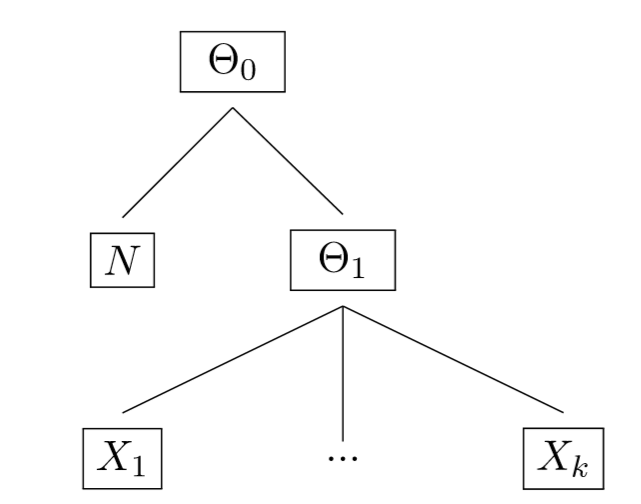
\includegraphics[height=5cm]{Hierarchie}
			\renewcommand{\figurename}{Illustration}
			\caption{Arbre hiérarchique à un niveau.} \label{graph_hierarchie}
		\end{figure}
	
		Ici, $\Theta_0$ représente une variable aléatoire définie sur $\mathbb{N}_+$ qui sert à créer un lien de dépendance entre la variable $N$ et les $\{X_i, i=1,\dots , k\}$. Ensuite, on a $\theta_1 = \sum_{i=1}^{\theta_0} B_i$ qui sert à créer un lien de dépendance entre les $X_i$. Les $B_i$ sont i.i.d. et indépendants de $\theta_0$. $B_i$ peut appartenir à $\mathbb{R}_+$ comme à $\mathbb{N}_+$. \\
		
		Sous cette représentation, on obtient une copule archimédienne hiérarchique s'exprimant comme
		
		\begin{equation}
		C(u_0, u_1, \dots, u_n) =
			\mathscr{L}_{\theta_0} \left(
				\mathscr{L}_{\theta_0}^{-1}(u_0) - \ln \left( 
					\mathscr{L}_B  \left(
						\sum_{i=1}^{n} \mathscr{L}_{B}^{-1} \left(
						 \exp \left(
						  - \mathscr{L}_{\theta_0}^{-1}(u_i) 
						  \right) \right)\right)\right)\right),
		\end{equation}
		où $\mathscr{L}$ correspond à la transformée de Laplace-Stieltjes d'une variable aléatoire.\\
		
		À ce point-ci, afin de trouver les paramètres d'une telle copule, il suffit d'appliquer \eqref{densite_composee} et \eqref{logLikelyhood}, puis d'optimiser numériquement.
		
	\section{Résultats}
		La présente section explique les scénarios testés ainsi que les résultats obtenus avec la méthodologie expliquée dans la section \ref{sect_Maxlikelyhood}.\\
		
		Pour les fins du présent travail, les estimations sont faites sur des données simulées. Pour faire ces simulations, le module \texttt{R} nommé \texttt{copula} \footnote{https://cran.r-project.org/web/packages/copula/copula.pdf}
		offre une fonction \texttt{rCopula} avec laquelle, il est possible de simuler différentes copules connues, dont la copule de Clayton. \\
		
		Pour les copules archimédiennes hiérarchique, le module \texttt{nCopula} \footnote{https://cran.r-project.org/web/packages/nCopula/nCopula.pdf} offre une fonction nommée \texttt{rCompCop} qui permet de simuler de la même façon que \texttt{rCopula}, mais en entrant comme argument la structure hiérarchique.
	
	\subsection{Copule de Clayton}
%		Scénario 1 : Binomial
		 \begin{Scenario}\label{scenario_Clayton_Binom}
			\textbf{Binomial}:
		 \end{Scenario}
	 
		 Pour débuter gentiment, prenons un modèle binomial-exponentiel avec une copule de Clayton dont la représentation est exprimée en \eqref{Copule_Clayton}.
		 Soient $N \sim Binom(n,q)$ et $X_i \sim X \sim Exp(\beta)$ et le paramètre de dépendance de la copule est dénotée $\alpha$.\\
	
		 Pour le premier scénario, on utilise des données simulées avec les paramètre initiaux présentés dans le tableau \ref{tbl_para_initiaux_Clayton_Binom}.
		 
		 \begin{table}[H]
		 	\centering
		 	\begin{tabular}{cccc}
		 		\hline
		 		$n$ & $q$ & $\alpha$ & $\beta$ \\ 
		 		\hline
		 		5.00 & 0.40 & 1.50 & 0.01 \\ 
		 		\hline
		 	\end{tabular}
	 	\caption{Paramètres initiaux pour la copule de Clayton avec $N \sim Bin(n, q),\ X_i \sim X \sim Exp(\beta)$.}
	 	\label{tbl_para_initiaux_Clayton_Binom}
		 \end{table}
		 
		Le sommaire des données simulées aux fins de l'estimation sont présentées dans le tableau \ref{tbl_sommaire_Clayton_Binom}. On y voit que la moyenne du nombre de sinistres est de 2 et que la moyenne des $x_i$ est très proche de 100; ce qui correspond aux attentes.
		De plus, les quantiles des $X_i$ sont très proches l'un de l'autre; ce qui signifie que les variables $X_i$ sont identiquement distribués. Visuellement parlant, l'illustration \ref{graph_densite_Binom} présente l'adéquation des données empiriques avec les lois théoriques. On voit donc que les variables simulées ont un comportement très similaire à la distribution marginale théorique des variables.\\
		
		% latex table generated in R 3.6.0 by xtable 1.8-4 package
		% Mon Jun 10 14:46:22 2019
		\begin{table}[H]
			\centering
			\begin{tabular}[width=\textwidth]{llllll}
				\hline
				       $N$ &       $X_1$ &       $X_2$ &             \\ 
				\hline
				 Min.   :0.000   & Min.   :  0.0049   & Min.   :   0.0066      \\ 
				 1st Qu.:1.000   & 1st Qu.: 28.8101   & 1st Qu.:  29.1251      \\ 
				 Median :2.000   & Median : 70.8847   & Median :  71.0354      \\ 
				 Mean   :1.991   & Mean   :101.0603   & Mean   : 101.3232      \\ 
				 3rd Qu.:3.000   & 3rd Qu.:140.7053   & 3rd Qu.: 139.3937      \\ 
				 Max.   :5.000   & Max.   :864.5799   & Max.   :1071.7262      \\ 
				\hline
			\end{tabular}
			%
			\begin{tabular}[width=\textwidth]{lll}
				\hline
				       $X_3$ &       $X_4$ &       $X_5$ \\ 
				\hline
			 	 Min.   :  0.0068   & Min.   :   0.0057   & Min.   :  0.007   \\ 
				 1st Qu.: 28.6798   & 1st Qu.:  29.1230   & 1st Qu.: 29.076   \\ 
				 Median : 69.3332   & Median :  70.2568   & Median : 69.112   \\ 
				 Mean   : 99.4368   & Mean   : 101.6533   & Mean   : 99.038   \\ 
				 3rd Qu.:137.4674   & 3rd Qu.: 141.3571   & 3rd Qu.:135.610   \\ 
				 Max.   :988.0162   & Max.   :1001.1827   & Max.   :840.130   \\ 
				\hline
			\end{tabular}
		\caption[Sommaire des données simulées pour le scénario \ref{scenario_Clayton_Binom}]{Sommaire de $10\,000$ simulations de $\{N, X_1, \dots, X_5\}$ en supposant que $F_{N,X_1,\dots, X_5}$ est définie avec une copule de Clayton($\alpha=1.5$), $N \sim Bin(5, 2/5)$ et $X_i \sim X \sim Exp(1/100)$, pour $i=1,\dots 5$.}
		\label{tbl_sommaire_Clayton_Binom}
		\end{table}
	
	
		\begin{figure}[H]
		\begin{subfigure}[l]{0.5\textwidth}
			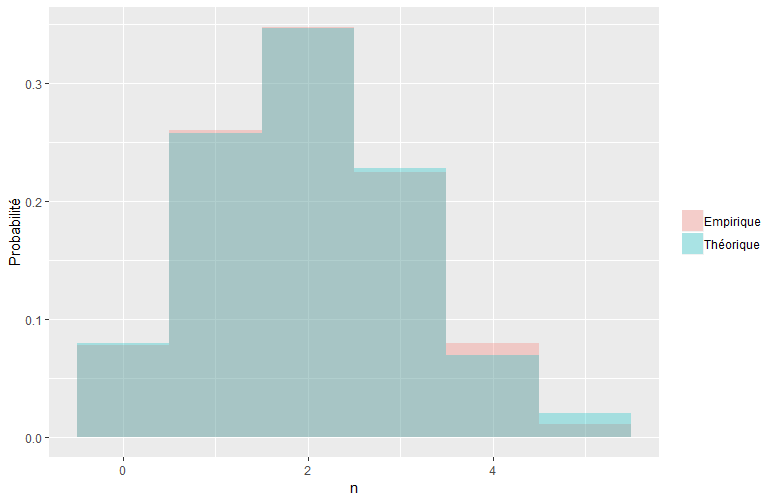
\includegraphics[width=\textwidth]{Graph/Clayton_Binom_N.png}
			\caption{Fréquence}
		\end{subfigure}
		%
		\begin{subfigure}[r]{0.5\textwidth}
			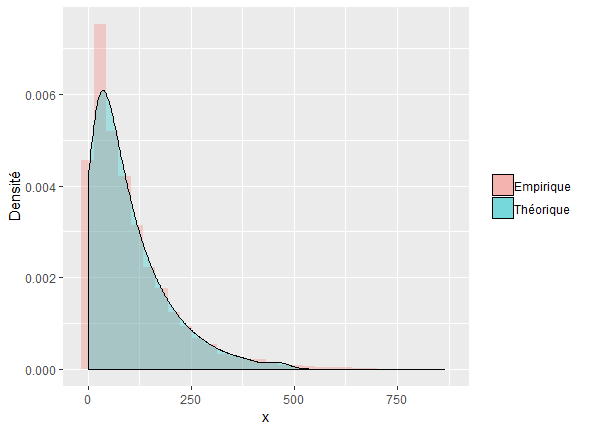
\includegraphics[width=\textwidth]{Graph/Clayton_Binom_X.png}
			\caption{Sévérité}
		\end{subfigure}
		\caption{Comparaisons de la distribution marginale des données simulées avec les distributions théoriques pour le scénario \ref{scenario_Clayton_Binom}.}
		\label{graph_densite_Binom}
		\end{figure}
		
		Pour ce qui est du comportement entre les variables, l'illustration \ref{graph_scatterplot_Binom} présente les nuages de points représentant les corrélations. On y voit que le $\rho$ de Spearman est le même pour tous les $X_i$. De plus, la forme des nuages de points pour les variables continues est caractéristique de la copule de Clayton. Cela indique que la simulation sort des résultats adéquats.\\
		
		\begin{figure}[H]
			\centering
			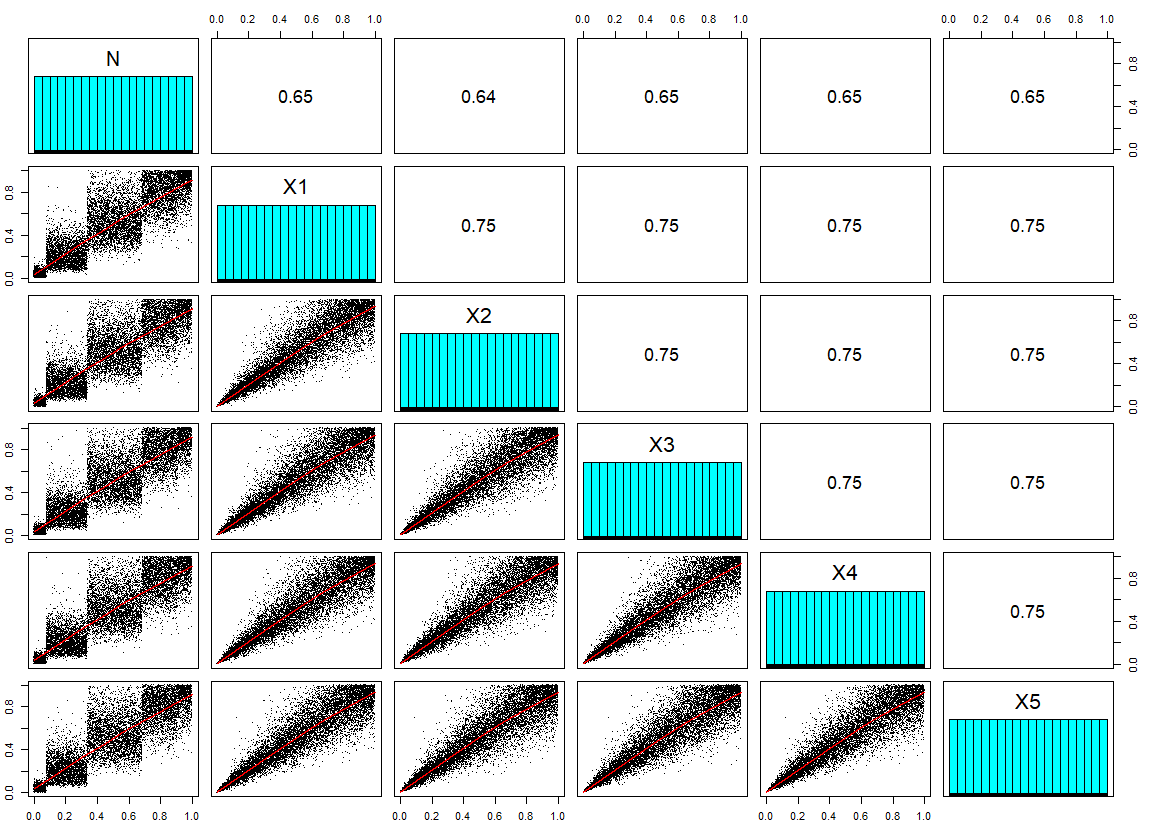
\includegraphics[height=10cm]{Graph/scatterplot_Binom.png}
			\caption[Nuages de points du scénario \ref{scenario_Clayton_Binom}]
			{Nuages de points avec copule de Clayton ($\alpha = 1.5$), $N\sim Binom(5,2/5)$ et $X_i \sim X\sim Exp(1/100)$:
				En bas de la diagonale se trouve les nuages de points illustrant la corrélation des différentes variables. En haut, on indique les coefficients de corrélation de Spearman. À noter que ce graphique est produit avec la fonction \texttt{R} \texttt{pairs.panels} du module \texttt{psych}. Dans cette dernière, le calcul des coefficients de corrélation sont calculés selon l'hypothèse que les variables sont continues. Cela implique que la première ligne n'est pas valide.}
			\label{graph_scatterplot_Binom}
		\end{figure}
		
		Avec les données simulées, on désire maintenant estimer les paramètres. On pose donc les valeurs de départ pour l'optimisation à l'estimateur du maximum de vraisemblance des distributions marginales des variables aléatoires. On a donc que $\tilde{q} = \bar{N}/n$, $\tilde{\beta} = 1/\bar{X}$, tel que $\bar{N}$ et $\bar{X}$ sont les moyennes empiriques de $N$ et $X$ respectivement. Pour ce qui est du $\alpha$ de la Clayton, il faut regarder les nuages de points de  l'illustration \ref{graph_scatterplot_Binom}. Plus le nuage est dense, plus le paramètre est grand. En revanche, si le nuage est large, plus $\alpha$ est près de 0.\\
		
		Pour ce scénario, on a comme valeur de départ $\tilde{q} = 0.398\,720, \tilde{\beta} = 0.010\,031$. Pour $\alpha$, posons la valeur initiale à 1. On obtient donc les estimateurs présentés dans le tableau \ref{tbl_Clayton_Binom}. On y voit que les résultats de l'estimation sont relativement très précises. De plus, pour une fréquence maximale de 5, les temps de dérivation et d'estimation sont très rapides.
		
		% latex table generated in R 3.6.0 by xtable 1.8-4 package
		% Mon Jun 10 14:54:45 2019
		\begin{table}[H]
			\centering
			\begin{tabular}{lrrr}
				\hline
				& $q$ & $\beta$ & $\alpha$ \\ 
				\hline
				Valeurs de départ & 0.3987 & 0.0100 & 1.0000 \\ 
				Estimateurs & 0.3997 & 0.0100 & 1.5051 \\ 
				Vrais paramètres & 0.4000 & 0.0100 & 1.5000 \\   
				\hline
			\end{tabular}
			%
			\begin{tabular}{lr}
				\hline
				&  \\ 
				\hline
				Temps de dérivation & 4.22  \\ 
				Temps d'estimation & 63.17  \\  
				\\
				\hline
			\end{tabular}
			\caption[Résultats du scénario \ref{scenario_Clayton_Binom}]{Résultats de l'estimation des paramètres avec une copule de Clayton($\alpha$), $N\sim Binom(n,q)$ et $X \sim Exp(\beta)$ suite à 10\,000 simulations.} 
			\label{tbl_Clayton_Binom}
		\end{table}
		
%		Scénario 2 : Poisson
		\begin{Scenario}\label{scenario_Clayton_Pois}
			\textbf{Poisson}:
		\end{Scenario}
	
		À la suite des résultats concluants du premier exemple, un modèle avec une loi de fréquence ayant un support infini peut ajouter un défi en terme de temps de calcul. Pour ce scénario, posons que $N \sim Pois(\lambda=1)$ et $X_i \sim X \sim Exp(\beta=1/100)$ et que le paramètre de dépendance de la Copule de Clayton est $\alpha = 1.5$. \\
		
		Comme pour le scénario \ref{scenario_Clayton_Binom}, un sommaire des données simulées est présenté dans le tableau \ref{tbl_sommaire_Clayton_Pois_1}, l'illustrations \ref{graph_scatterplot_Poiss_1} compare la distribution marginale des données empiriques avec celle des lois théorique et l'illustration \ref{graph_scatterplot_Poiss_1} présente les nuages de points afin de voir les corrélations.
		
		% latex table generated in R 3.6.0 by xtable 1.8-4 package
		% Mon Jun 10 10:40:57 2019
		\begin{table}[H]
			\centering
			\begin{tabular}{lllll}
				\hline
				       $N$ &      $X_1$ &      $X_2$ &       $X_3$ &       $X_4$ \\
				\hline
				  Min.   :0.0000   & Min.   :  0.006   & Min.   :   0.0076   & Min.   :   0.004   & Min.   :  0.0047      \\ 
				  1st Qu.:0.0000   & 1st Qu.: 29.296   & 1st Qu.:  28.6055   & 1st Qu.:  29.217   & 1st Qu.: 28.8844      \\ 
				  Median :1.0000   & Median : 68.978   & Median :  70.1421   & Median :  70.539   & Median : 69.1708      \\ 
				  Mean   :0.9987   & Mean   : 99.922   & Mean   : 100.1551   & Mean   :  99.760   & Mean   : 98.9900      \\ 
				  3rd Qu.:2.0000   & 3rd Qu.:138.052   & 3rd Qu.: 136.9883   & 3rd Qu.: 137.060   & 3rd Qu.:136.3721      \\ 
				  Max.   :6.0000   & Max.   :914.272   & Max.   :1041.9811   & Max.   :1050.119   & Max.   :953.2574      \\ 
				 \hline
			\end{tabular}
	
			\begin{tabular}{llll}
				\hline
				$X_5$ &      $X_6$ &       $X_7$ &       $X_8$ \\ 
				\hline
				 Min.   :   0.0068   & Min.   :  0.008   & Min.   :  0.0072   & Min.   :  0.0093   \\ 
				 1st Qu.:  29.5422   & 1st Qu.: 28.664   & 1st Qu.: 29.3327   & 1st Qu.: 28.8089   \\ 
				 Median :  70.7936   & Median : 71.331   & Median : 69.5485   & Median : 69.3149   \\ 
				 Mean   : 100.4916   & Mean   :102.201   & Mean   :101.1266   & Mean   : 99.5730   \\ 
				 3rd Qu.: 139.2436   & 3rd Qu.:141.000   & 3rd Qu.:139.8154   & 3rd Qu.:137.2429   \\ 
				 Max.   :1078.6322   & Max.   :894.636   & Max.   :961.4753   & Max.   :824.4899   \\ 
				\hline
		\end{tabular}
		\caption[Sommaire des données simulées pour le scénario \ref{scenario_Clayton_Pois}]{Sommaire de $10\,000$ simulations de $\{N, X_1, \dots, X_8\}$ en supposant que $F_{N,X_1,\dots, X_8}$ est définie avec une copule de Clayton($\alpha=1.5$), $N \sim Pois(1)$ et $X_i \sim X \sim Exp(1/100)$, pour $i=1,\dots 8$.}\label{tbl_sommaire_Clayton_Pois_1}
		\end{table}
		
		\begin{figure}[H]
			\begin{subfigure}[l]{0.5\textwidth}
				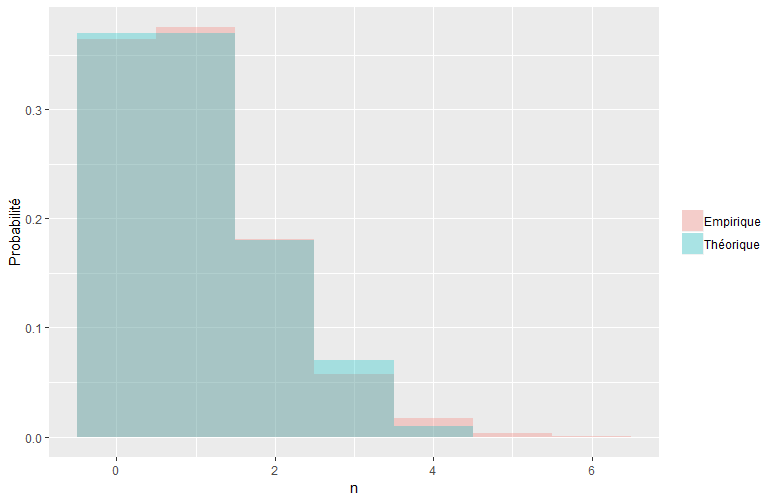
\includegraphics[width=\textwidth]{Graph/Clayton_Poiss_1_N.png}
				\caption{Fréquence}
			\end{subfigure}
			%
			\begin{subfigure}[r]{0.5\textwidth}
				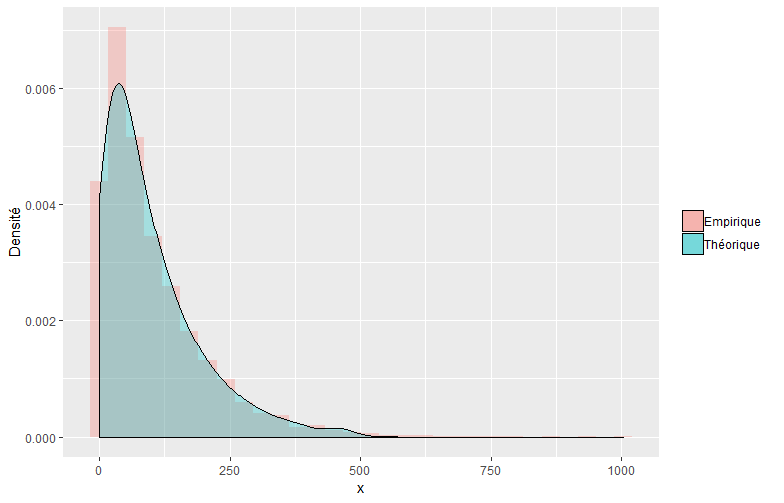
\includegraphics[width=\textwidth]{Graph/Clayton_Poiss_1_X.png}
				\caption{Sévérité}
			\end{subfigure}
			\caption{Comparaisons de la distribution marginale des données simulées avec les distributions théoriques pour le scénario \ref{scenario_Clayton_Pois}.}\label{graph_densite_Poisson_1}
		\end{figure}
	
		\begin{figure}[H]
			\centering
			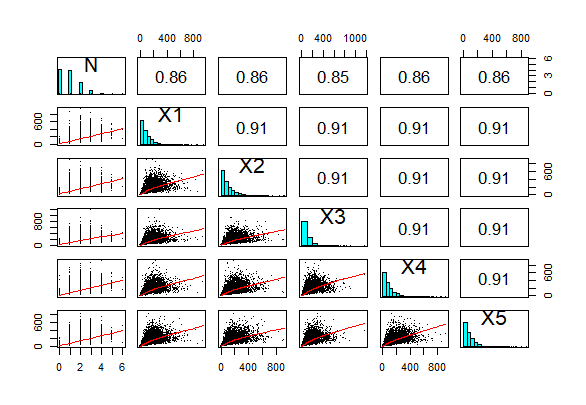
\includegraphics[height=10cm]{Graph/scatterplot_Poisson_1.png}
			\caption[Nuages de points du scénario \ref{scenario_Clayton_Pois}]{Nuages de points avec copule de Clayton ($\alpha = 1.5$), $N\sim Pois(1)$ et $X_i \sim X\sim Exp(1/100)$:
			En bas de la diagonale se trouve les nuages de points illustrant la corrélation des différentes variables. En haut, on indique les coefficients de corrélation de Spearman. À noter que ce graphique est produit avec la fonction \texttt{R} \texttt{pairs.panels} du module \texttt{psych}. Dans cette dernière, le calcul des coefficients de corrélation sont calculés selon l'hypothèse que les variables sont  continues. Cela implique que la première ligne n'est pas valide.} 
			\label{graph_scatterplot_Poiss_1}
		\end{figure}
	
		Comme pour le scénario \ref{scenario_Clayton_Binom}, le tableau \ref{tbl_sommaire_Clayton_Pois_1} et les illustrations \ref{graph_scatterplot_Poiss_1} démontrent que les résultats de la simulation sont adéquats.\\
		
		Pour ce qui est de l'estimation des paramètres, commençons par définir les paramètres initiaux. On pose donc $\tilde{\lambda} = \bar{N} = 0.998\,700, \tilde{\beta} = 1/\bar{X}= 0.009\,972$ et comme pour l'exemple précédent, prenons 1 comme valeur de départ pour $\alpha$. Les estimations obtenus sont présentés dans le tableau \ref{tbl_Clayton_Poisson}.
		
		% latex table generated in R 3.6.0 by xtable 1.8-4 package
		% Thu Jun 06 16:25:40 2019
		\begin{table}[H]
			\centering
			\begin{tabular}{lrrr}
				\hline
				& $\lambda$ & $\beta$ & $\alpha$ \\ 
				\hline
				Valeurs de départ & 0.9987 & 0.0100 & 1.0000 \\ 
				Estimateurs & 1.0040 & 0.0101 & 1.5415 \\ 
				Vrais paramètres & 1.0000 & 0.0100 & 1.5000 \\
				\hline
			\end{tabular}
	%	
		\begin{tabular}{lr}
			\hline
			&  \\ 
			\hline
			Temps de dérivation & 12.60 \\ 
			Temps d'estimation & 75.27 \\ 
			\\
			\hline
		\end{tabular}
			\caption[Résultats du scénario \ref{scenario_Clayton_Pois}]{Résultats de l'estimation des paramètres avec une copule de Clayton($\alpha$), $N\sim Pois(\lambda)$ et $X \sim Exp(\beta)$ suite à 10\,000 simulations.}\label{tbl_Clayton_Poisson}
		\end{table}
	
		Dans cet exemple, l'estimation n'est pas plus longue puisque le paramètre de la poisson n'est pas très grand. Cependant, si on l'augmente un tant soit peu, on obtient des quantiles élevés qui font en sorte que le temps de dérivation augmente de façon exponentielle.\\
	
		Par exemple, si $N \sim Pois(2)$, le temps de calcul dépasse 12 heures puisque le 99,9999 percentile de cette loi est de 12. Ainsi la méthode du maximum de vraisemblance nécessite de générer une liste de douze fonctions qui sont dérivées jusqu'à douze fois. Même avec la fonction \texttt{Deriv} de \texttt{R}, ce processus est extrêmement long. À cet effet, l'illustration \ref{graph_temps_deriv} présente le temps de dérivation selon le nombre de dérivées partielles à effectuer sur une copule de Clayton.
		
		\begin{figure}[H]
			\centering
			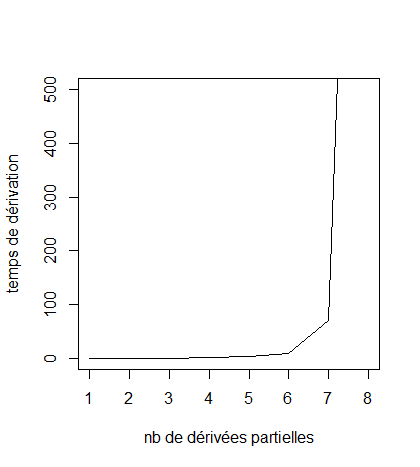
\includegraphics[height=8cm]{Graph/graph_temps_deriv.png}
			\caption{Temps de dérivation d'une copule de Clayton en fonction du nombre de dérivées partielles à effectuer.}
			\label{graph_temps_deriv}
		\end{figure}
		
			
		Ce que l'on peut observer avec ces deux résultats, c'est, d'une part, qu'avec 10\,000 simulations, on obtient des résultats très adéquats. D'autre part, on peut observer que le temps de calcul augmente significativement si $N$ peut prendre des valeurs supérieures à 7 et si le nombre de paramètres à estimer est grand. Le temps de calcul est donc un enjeu important.

	\subsection{Copule archimédienne hiérarchique}
		Désormais, prenons la copule qui nous intéresse vraiment: la copule archimédienne hiérarchique. Dans la présente section un scénario est fait pour chacune des six familles de copule archimédienne hiérarchique.\\
		
% Scénario 3 : Logarithmique-logarithmique
		\begin{Scenario}\label{scenario_log_log}
			\textbf{Logarithmique-Logarithmique}
		\end{Scenario}
	
		Soit $\Theta_0 \sim Logarithmique(\gamma_0)$ avec $\mathscr{L}_{\Theta_0} = \frac{\ln(1-\gamma_0 e^{-t})}{\ln(1-\gamma_0)}$ et $\mathscr{L}^{-1}_{\Theta_0} = -\ln \left( \frac{1-(1-\gamma_0)^u}{\gamma_0} \right)$.
		%
		Soit $B_i \sim B \sim Logarithmique(\gamma_1)$ avec $\mathscr{L}_{B} = \frac{\ln(1-\gamma_1 e^{-t})}{\ln(1-\gamma_1)}$ et $\mathscr{L}^{-1}_{B} = -\ln \left( \frac{1-(1-\gamma_1)^u}{\gamma_1} \right)$. Soient $\alpha_{0} = -ln(1-\gamma_0)$ et $\alpha_{1} = -ln(1-\gamma_1)$. Avec $\alpha_0 = 0.5$, $\alpha_1 = 0.8$, $N\sim Bin(n=5, q=2/5)$ et $X_i \sim X \sim Exp(\beta = 1/100)$, on obtient le sommaire des simulations présenté dans le tableau \ref{tbl_sommaire_log_log} ainsi que les illustrations \ref{graph_densite_log_log} et \ref{graph_scatterplot_log_log}.
		
		% latex table generated in R 3.6.0 by xtable 1.8-4 package
		% Wed Jun 12 11:29:43 2019
		\begin{table}[H]
			\centering
			\begin{tabular}{lll}
				\hline
				      $N$ &       $X_1$ &       $X_2$  \\ 
				\hline
				 Min.   :0.000   & Min.   :   0.0005   & Min.   :   0.0003    \\ 
				 1st Qu.:1.000   & 1st Qu.:  28.8718   & 1st Qu.:  28.7527      \\ 
				 Median :2.000   & Median :  70.2264   & Median :  69.5752     \\ 
				 Mean   :1.993   & Mean   :  99.0743   & Mean   : 101.3211      \\ 
				 3rd Qu.:3.000   & 3rd Qu.: 137.8503   & 3rd Qu.: 140.6853     \\ 
				 Max.   :5.000   & Max.   :1159.3514   & Max.   :1276.8609     \\ 
				\hline
			\end{tabular}
		%
			\begin{tabular}{lll}
				\hline
				       $X_3$ &      $X_4$&       $X_5$ \\ 
				\hline
				 Min.   :  0.0039   & Min.   :  0.0003   & Min.   :  0.0055   \\ 
				 1st Qu.: 27.8579   & 1st Qu.: 29.2991   & 1st Qu.: 28.8589   \\ 
				 Median : 69.3043   & Median : 69.3083   & Median : 69.9943   \\ 
				 Mean   : 99.3564   & Mean   : 99.3880   & Mean   :100.8576   \\ 
				 3rd Qu.:138.5018   & 3rd Qu.:136.2992   & 3rd Qu.:140.1445   \\ 
				 Max.   :867.0918   & Max.   :852.5330   & Max.   :997.9467   \\ 
				\hline
			\end{tabular}
		\caption[Sommaire des données simulées pour le scénario \ref{scenario_log_log}]{Sommaire de $10\,000$ simulations de $\{N, X_1, \dots, X_5\}$ en supposant que $F_{N,X_1,\dots, X_5}$ est définie avec une copule de archimédienne hiérarchique logarithmique-logarithmique($\alpha_0=0.5, \alpha_1=0.8$), $N \sim Bin(5, 2/5)$ et $X_i \sim X \sim Exp(1/100)$, pour $i=1,\dots, 5$.}
		\label{tbl_sommaire_log_log}
		\end{table}
	
		\begin{figure}[H]
			\begin{subfigure}[l]{0.5\textwidth}
				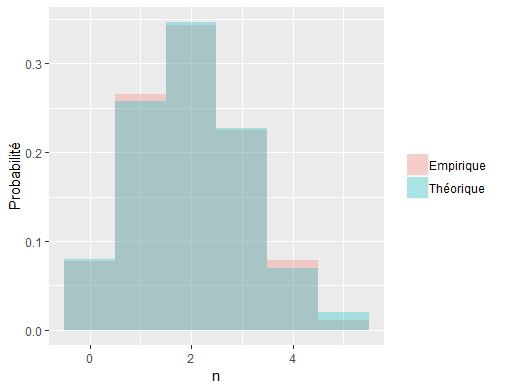
\includegraphics[width=\textwidth]{Graph/log_log_N.png}
				\caption{Fréquence}
			\end{subfigure}
			%
			\begin{subfigure}[r]{0.5\textwidth}
				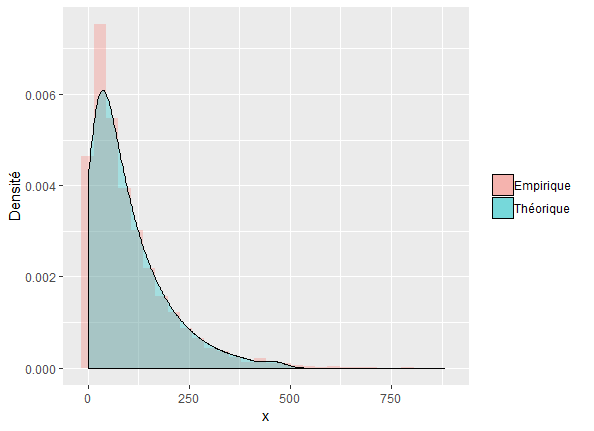
\includegraphics[width=\textwidth]{Graph/log_log_X.png}
				\caption{Sévérité}
			\end{subfigure}
			\caption{Comparaisons de la distribution marginale des données simulées avec les distributions théoriques pour le scénario \ref{scenario_log_log}.}
			\label{graph_densite_log_log}
		\end{figure}
	
		\begin{figure}[H]
			\centering
			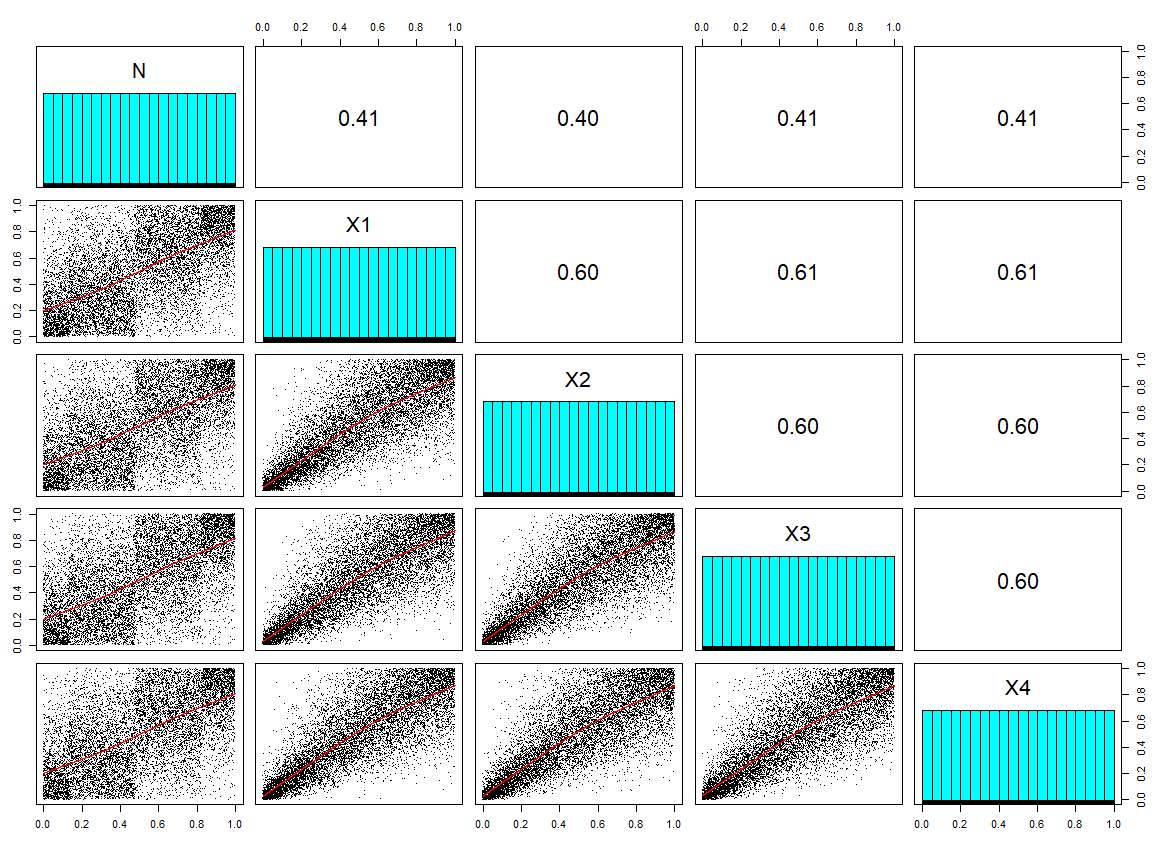
\includegraphics[height=10cm]{Graph/scatterplot_log_log.png}
			\caption[Nuages de points du scénario \ref{scenario_log_log}]
			{Nuages de points avec copule archimédienne hiérarchique logarithmique-logarithmique($\alpha_0=0.5, \alpha_1=0.8$), $N \sim Bin(5, 2/5)$ et $X_i \sim X \sim Exp(1/100)$, pour $i=1,\dots, 5$.:
				En bas de la diagonale se trouve les nuages de points illustrant la corrélation des différentes variables. En haut, on indique les coefficients de corrélation de Spearman. À noter que ce graphique est produit avec la fonction \texttt{R} \texttt{pairs.panels} du module \texttt{psych}. Dans cette dernière, le calcul des coefficients de corrélation sont calculés selon l'hypothèse que les variables sont continues. Cela implique que la première ligne n'est pas valide.}
			\label{graph_scatterplot_log_log}
		\end{figure}
		
		Pour l'estimation des paramètres initiaux, avec la méthode du maximum de vraisemblance, on a $\tilde{q} = \bar{N}/n = 0.398\,600$ et $\tilde{\beta} = 1/\bar{X} = 0.010\,070$. Cependant, pour les paramètres de dépendance, il n'est pas aisé de trouver des valeurs de départ adéquates. Pour le moment, de façon arbitraire, posons $\alpha_{0}=\alpha_{1}=0.4$. On obtient donc les estimateurs présentés dans le tableau \ref{tbl_resultats_log_log}
		
		% latex table generated in R 3.6.0 by xtable 1.8-4 package
		% Wed Jun 12 11:40:24 2019
		\begin{table}[H]
			\centering
			\begin{tabular}{lrrrr}
				\hline
				& $q$ & $\beta$ & $\alpha_0$ & $\alpha_1$ \\ 
				\hline
				Valeurs de départ & 0.3986 & 0.0100 & 0.4000 & 0.4000 \\ 
				Estimateurs & 0.3986 & 0.0100 & 0.4499 & 0.7700 \\ 
				Vrais paramètres & 0.4000 & 0.0100 & 0.5000 & 0.8000 \\ 
				\hline
			\end{tabular}
		%
			\begin{tabular}{lr}
				\hline
				&  \\ 
				\hline
				Temps de dérivation & 2199.69 \\ 
				Temps d'estimation & 254.75 \\ 
				\\
				\hline
			\end{tabular}
		\caption[Résultats du scénario \ref{scenario_log_log}]{Résultats de l'estimation des paramètres avec une copule archimédienne hiérarchique logarithmique-logarithmique($\alpha_0=0.5, \alpha_1=0.8$), $N \sim Bin(5, 2/5)$ et $X_i \sim X \sim Exp(1/100)$, pour $i=1,\dots, 5$, à la suite de 10\,000 simulations.}
		\label{tbl_resultats_log_log}
		\end{table}
	
		À la lecture du tableau \ref{tbl_resultats_log_log}, on voit que les estimateurs de $\alpha_0$ et $\alpha_1$ sont moins près des vrais valeurs que pour les autres. Cela est explicable du fait que, pour ces paramètres, les valeurs de départ ne sont pas optimales ce qui augmente les probabilités que la fonction \texttt{R} \texttt{constrOptim} ne trouve pas le minimum absolu de la fonction de score, mais plutôt qu'elle trouve un minimum local.
		
% Scénario 4 : Logarithmique-gamma
		\begin{Scenario}\label{scenario_log_gamma}
			\textbf{Logarithmique-Gamma}
		\end{Scenario}
	
		Soit $\Theta_0 \sim Logarithmique(\gamma)$ avec $\mathscr{L}_{\Theta_0} = \frac{\ln(1-\gamma e^{-t})}{\ln(1-\gamma)}$ et $\mathscr{L}^{-1}_{\Theta_0} = -\ln \left( \frac{1-(1-\gamma)^u}{\gamma} \right)$. Soit $\alpha_{0} = -ln(1-\gamma)$.
		%
		Soit $B_i \sim B \sim gamma(1/\alpha_1,1)$ avec $\mathscr{L}_{B} = (1+t)^{-1/\alpha_1}$ et $\mathscr{L}^{-1}_{B} = u^{-\alpha_1} - 1$. Avec $\alpha_0 = 0.5$, $\alpha_1 = 5$, $N\sim Bin(n=5, q=2/5)$ et $X_i \sim X \sim Exp(\beta = 1/100)$, on obtient le sommaire des simulations présenté dans le tableau \ref{tbl_sommaire_log_gamma} ainsi que les illustrations \ref{graph_densite_log_gamma} et \ref{graph_scatterplot_log_gamma}.
		
		\begin{table}[H]
			\centering
			\begin{tabular}{lll}
				\hline
				       $N$ &       $X_1$ &       $X_2$        \\ 
				\hline
				  Min.   :0   & Min.   :  0.0114   & Min.   :   0.0121    \\ 
				  1st Qu.:1   & 1st Qu.: 28.3559   & 1st Qu.:  27.984    \\ 
				  Median :2   & Median : 68.5183   & Median :  67.6682   \\ 
				  Mean   :2   & Mean   : 98.2412   & Mean   :  99.0285    \\ 
				  3rd Qu.:3   & 3rd Qu.:136.8315   & 3rd Qu.: 138.0584      \\ 
				  Max.   :5   & Max.   :888.6908   & Max.   :1008.9367     \\ 
				\hline
			\end{tabular}
		%
			\begin{tabular}{lll}
				\hline
				          $X_3$ &       $X_4$ &       $X_5$ \\ 
				\hline
				  Min.   :  0.0113   & Min.   :  0.0273   & Min.   :   0.0118   \\ 
				  1st Qu.: 28.1662   & 1st Qu.: 28.0790   & 1st Qu.:  28.1698   \\ 
				  Median : 69.8290   & Median : 68.1602   & Median :  68.6309   \\ 
				  Mean   : 99.3519   & Mean   : 98.5785   & Mean   :  98.8991   \\ 
				  3rd Qu.:139.2965   & 3rd Qu.:138.2672   & 3rd Qu.: 136.6441   \\ 
				  Max.   :781.9900   & Max.   :950.1376   & Max.   :1095.3264   \\
				\hline
			\end{tabular}
		\caption[Sommaire des données simulées pour le scénario \ref{scenario_log_gamma}]{Sommaire de $10\,000$ simulations de $\{N, X_1, \dots, X_5\}$ en supposant que $F_{N,X_1,\dots, X_5}$ est définie avec une copule de archimédienne hiérarchique logarithmique-gamma($\alpha_0=0.5, \alpha_1 = 5$), $N \sim Bin(5, 2/5)$ et $X_i \sim X \sim Exp(1/100)$, pour $i=1,\dots, 5$.}
		\label{tbl_sommaire_log_gamma}
		\end{table}
		
		\begin{figure}[H]
			\begin{subfigure}[l]{0.5\textwidth}
				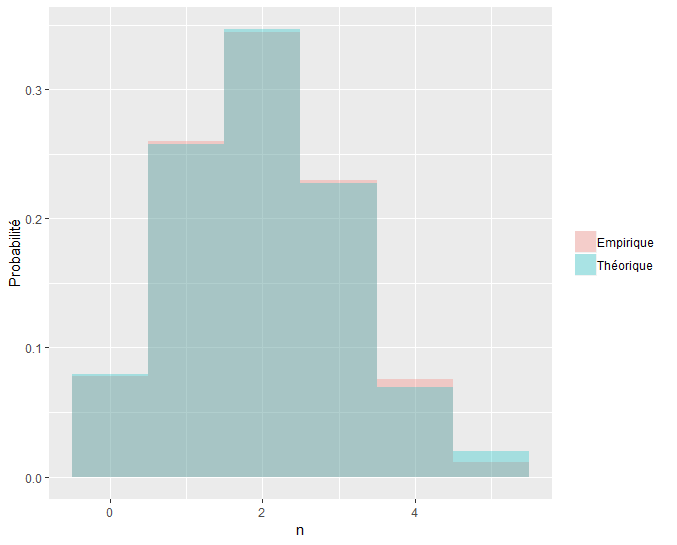
\includegraphics[width=\textwidth]{Graph/log_gamma_N.png}
				\caption{Fréquence}
			\end{subfigure}
			%
			\begin{subfigure}[r]{0.5\textwidth}
				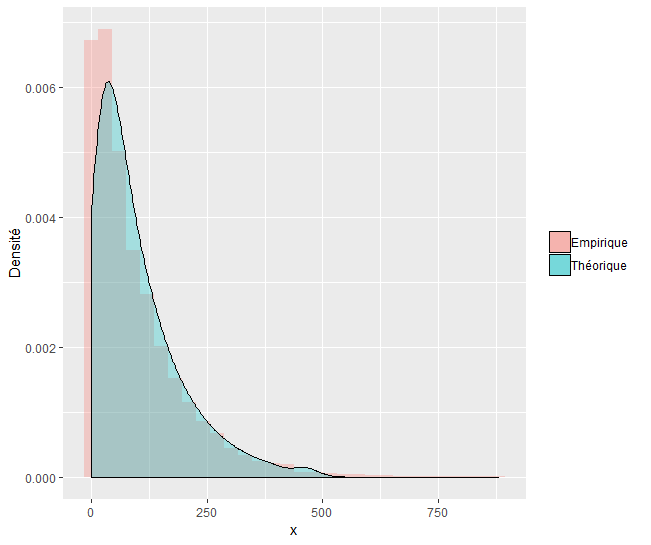
\includegraphics[width=\textwidth]{Graph/log_gamma_X.png}
				\caption{Sévérité}
			\end{subfigure}
			\caption{Comparaisons de la distribution marginale des données simulées avec les distributions théoriques pour le scénario \ref{scenario_log_gamma}.}
			\label{graph_densite_log_gamma}
		\end{figure}
		
		\begin{figure}[H]
			\centering
			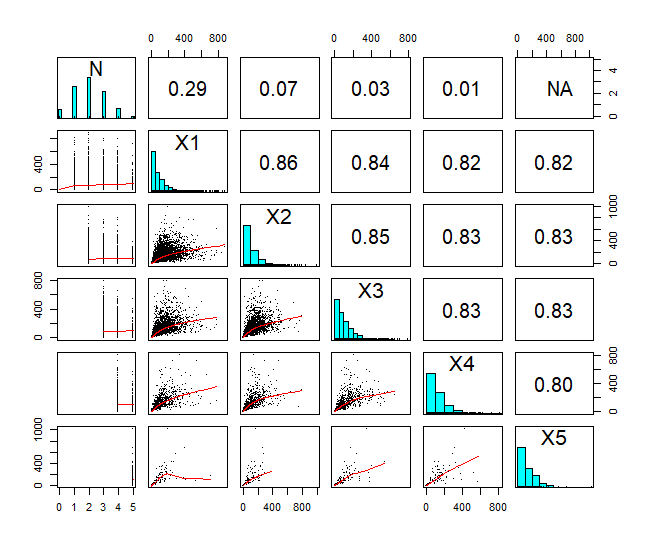
\includegraphics[height=10cm]{Graph/scatterplot_log_gamma.png}
			\caption[Nuages de points du scénario \ref{scenario_log_gamma}]
			{Nuages de points avec copule archimédienne hiérarchique logarithmique-gamma($\alpha_0=0.5, \alpha_1 = 5$), $N \sim Bin(5, 2/5)$ et $X_i \sim X \sim Exp(1/100)$, pour $i=1,\dots, 5$.:
				En bas de la diagonale se trouve les nuages de points illustrant la corrélation des différentes variables. En haut, on indique les coefficients de corrélation de Spearman. À noter que ce graphique est produit avec la fonction \texttt{R} \texttt{pairs.panels} du module \texttt{psych}. Dans cette dernière, le calcul des coefficients de corrélation sont calculés selon l'hypothèse que les variables sont continues. Cela implique que la première ligne n'est pas valide.}
			\label{graph_scatterplot_log_gamma}
		\end{figure}

		Les valeurs de départ de l'optimisation numérique ainsi que les résultats de l'estimation sont présentés dans le tableau \ref{tbl_resultats_log_gamma}.
	
		\begin{table}[H]
			\centering
			\begin{tabular}{lrrrr}
				\hline
				& $q$ & $\beta$ & $\alpha_0$ & $\alpha_1$ \\ 
				\hline
				Valeurs de départ & 0.4001 & 0.0097 & 0.5000 & 4.0000 \\ 
				Estimateurs & 0.3970  &0.00983 & 0.5133 &  5.0751 \\ 
				Vrais paramètres & 0.4000 & 0.0100 & 0.5000 & 5.0000 \\
				\hline
			\end{tabular}
			%
			\begin{tabular}{lr}
				\hline
				&  \\ 
				\hline
				Temps de dérivation & 50.38  \\ 
				Temps d'estimation & 2714.00 \\ 
				\\
				\hline
			\end{tabular}
			\caption[Résultats du scénario \ref{scenario_log_gamma}]{Résultats de l'estimation des paramètres avec une copule archimédienne hiérarchique logarithmique-gamma($\alpha_0=0.5, \alpha_1=5$), $N \sim Bin(5, 2/5)$ et $X_i \sim X \sim Exp(1/100)$, pour $i=1,\dots,5$, à la suite de 10\,000 simulations.}
			\label{tbl_resultats_log_gamma}
		\end{table}
	
	
% Scénario 5: Logarithmique-geo
	\begin{Scenario}\label{scenario_log_geo}
		\textbf{Logarithmique-Géométrique}
	\end{Scenario}
	
	Soit $\Theta_0 \sim Logarithmique(\gamma)$ avec $\mathscr{L}_{\Theta_0} = \frac{\ln(1-\gamma e^{-t})}{\ln(1-\gamma)}$ et $\mathscr{L}^{-1}_{\Theta_0} = -\ln \left( \frac{1-(1-\gamma)^u}{\gamma} \right)$. Soit $\alpha_{0} = -ln(1-\gamma)$.
	%
	Soit $B_i \sim B \sim Geo(1-\alpha_1)$ avec $E[B] = \frac{1}{1-\alpha_1},\ \mathscr{L}_{B} = \frac{1-\alpha_1}{e^t-\alpha_1}$ et $\mathscr{L}^{-1}_{B} = \ln\left(\frac{1 - \alpha_1}{u}+\alpha_1\right)$. Avec $\alpha_0 = 0.5$, $\alpha_1 = 0.3$, $N\sim Bin(n=5, q=2/5)$ et $X_i \sim X \sim Exp(\beta = 1/100)$, on obtient le sommaire des simulations présenté dans le tableau \ref{tbl_sommaire_log_geo} ainsi que les illustrations \ref{graph_densite_log_geo} et \ref{graph_scatterplot_log_geo}.
	
	\begin{table}[H]
		\centering
		\begin{tabular}{lll}
			\hline
			$N$ &       $X_1$ &       $X_2$        \\ 
			\hline
			  Min.   :0.000   & Min.   :  0.0152   & Min.   :  0.0023      \\ 
			  1st Qu.:1.000   & 1st Qu.: 28.3205   & 1st Qu.: 27.6623      \\ 
			  Median :2.000   & Median : 68.6348   & Median : 68.6183       \\ 
			  Mean   :1.994   & Mean   : 98.9724   & Mean   : 98.2568      \\ 
			  3rd Qu.:3.000   & 3rd Qu.:138.8460   & 3rd Qu.:136.5162       \\ 
			  Max.   :5.000   & Max.   :959.2391   & Max.   :857.1796      \\
			\hline
		\end{tabular}
		%
		\begin{tabular}{lll}
			\hline
			$X_3$ &       $X_4$ &       $X_5$ \\ 
			\hline
			  Min.   :   0.0015   & Min.   :  0.0052   & Min.   :  0.0033   \\ 
			  1st Qu.:  28.5541   & 1st Qu.: 29.3939   & 1st Qu.: 28.1749   \\ 
			  Median :  68.5017   & Median : 71.0794   & Median : 68.6236   \\ 
			  Mean   : 100.1266   & Mean   :100.1761   & Mean   : 97.9566   \\ 
			  3rd Qu.: 138.9653   & 3rd Qu.:138.0791   & 3rd Qu.:136.7516   \\ 
			  Max.   :1195.4707   & Max.   :754.0023   & Max.   :924.5513   \\ 
			\hline
		\end{tabular}
		\caption[Sommaire des données simulées pour le scénario \ref{scenario_log_geo}]{Sommaire de $10\,000$ simulations de $\{N, X_1, \dots, X_5\}$ en supposant que $F_{N,X_1,\dots, X_5}$ est définie avec une copule de archimédienne hiérarchique logarithmique-géométrique($\alpha_0=0.5, \alpha_1 = 0.3$), $N \sim Bin(5, 2/5)$ et $X_i \sim X \sim Exp(1/100)$, pour $i=1,\dots, 5$.}
		\label{tbl_sommaire_log_geo}
	\end{table}
	
	\begin{figure}[H]
		\begin{subfigure}[l]{0.5\textwidth}
			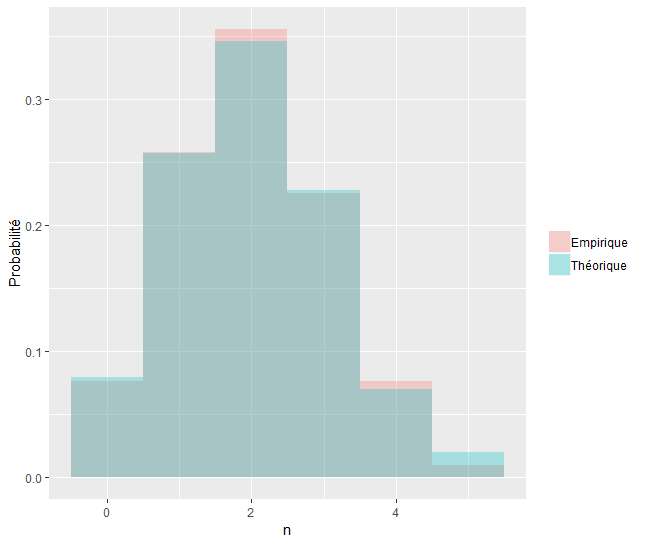
\includegraphics[width=\textwidth]{Graph/log_geo_N.png}
			\caption{Fréquence}
		\end{subfigure}
		%
		\begin{subfigure}[r]{0.5\textwidth}
			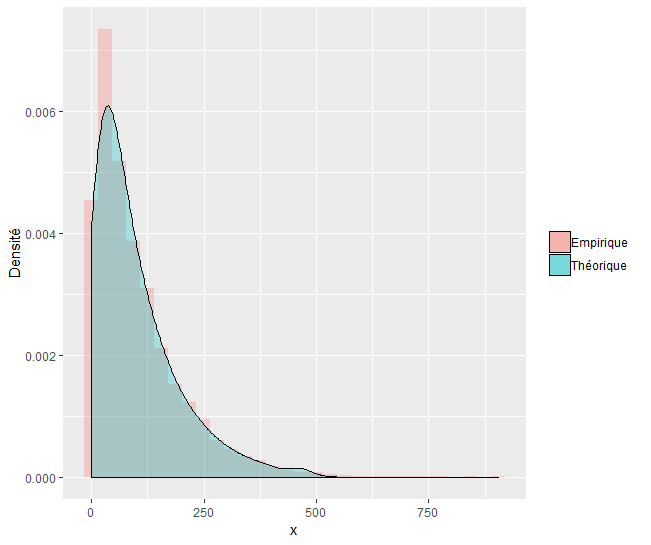
\includegraphics[width=\textwidth]{Graph/log_geo_X.png}
			\caption{Sévérité}
		\end{subfigure}
		\caption{Comparaisons de la distribution marginale des données simulées avec les distributions théoriques pour le scénario \ref{scenario_log_geo}.}
		\label{graph_densite_log_geo}
	\end{figure}
	
	\begin{figure}[H]
		\centering
		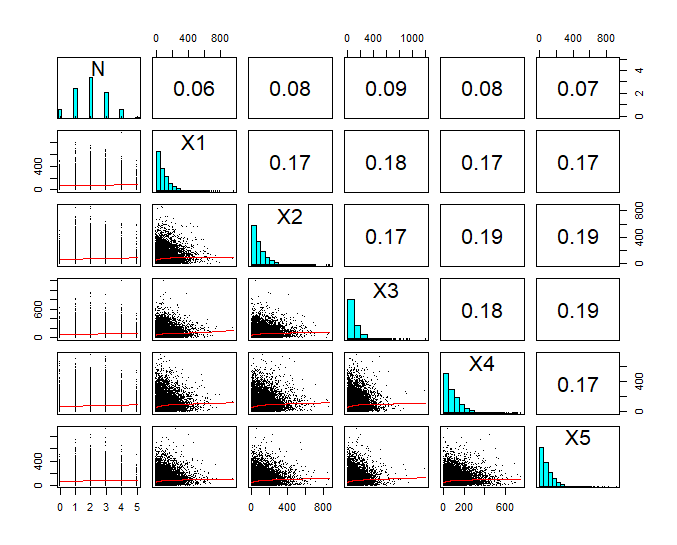
\includegraphics[height=10cm]{Graph/scatterplot_log_geo.png}
		\caption[Nuages de points du scénario \ref{scenario_log_geo}]
		{Nuages de points avec copule archimédienne hiérarchique logarithmique-géométrique($\alpha_0=0.5, \alpha_1 = 0.3$), $N \sim Bin(5, 2/5)$ et $X_i \sim X \sim Exp(1/100)$, pour $i=1,\dots, 5$.:
			En bas de la diagonale se trouve les nuages de points illustrant la corrélation des différentes variables. En haut, on indique les coefficients de corrélation de Spearman. À noter que ce graphique est produit avec la fonction \texttt{R} \texttt{pairs.panels} du module \texttt{psych}. Dans cette dernière, le calcul des coefficients de corrélation sont calculés selon l'hypothèse que les variables sont continues. Cela implique que la première ligne n'est pas valide.}
		\label{graph_scatterplot_log_geo}
	\end{figure}
	
	Les valeurs de départ de l'optimisation numérique ainsi que les résultats de l'estimation sont présentés dans le tableau \ref{tbl_resultats_log_geo}.
	
	\begin{table}[H]
		\centering
		\begin{tabular}{lrrrr}
			\hline
			& $q$ & $\beta$ & $\alpha_0$ & $\alpha_1$ \\ 
			\hline
			Valeurs de départ & 0.3987 & 0.0097 & 0.5000 & 0.5000 \\ 
			Estimateurs & 0.3999 & 0.0100 & 0.5028 & 0.5059 \\ 
			Vrais paramètres & 0.4000 & 0.0100 & 0.5000 & 0.3000 \\
			\hline
		\end{tabular}
		%
		\begin{tabular}{lr}
			\hline
			&  \\ 
			\hline
			Temps de dérivation & 109.45 \\ 
			Temps d'estimation & 1001.81 \\ 
			\\
			\hline
		\end{tabular}
		\caption[Résultats du scénario \ref{scenario_log_geo}]{Résultats de l'estimation des paramètres avec une copule archimédienne hiérarchique logarithmique-géométrique($\alpha_0=0.5, \alpha_1 = 0.3$), $N \sim Bin(5, 2/5)$ et $X_i \sim X \sim Exp(1/100)$, pour $i=1,\dots,5$, à la suite de 10\,000 simulations.}
		\label{tbl_resultats_log_geo}
	\end{table}



% Scénario 6: geo-logarithmic
	\begin{Scenario}\label{scenario_geo_log}
		\textbf{Géométrique-Logarithmique}
	\end{Scenario}
	
	Soit $\Theta_0 \sim Geo(1-\alpha_0)$ avec $E[M] = \frac{1}{1-\alpha_0},\ \mathscr{L}_{\Theta_0} = \frac{1-\alpha_0}{e^t-\alpha_0}$ et $\mathscr{L}^{-1}_{\Theta_0} = \ln\left(\frac{1 - \alpha_0}{u}+\alpha_0\right)$.
	%
	Soit $B_i \sim B \sim Logarithmique(\gamma)$ avec $\mathscr{L}_{B} = \frac{\ln(1-\gamma e^{-t})}{\ln(1-\gamma)}$ et $\mathscr{L}^{-1}_{B} = -\ln \left( \frac{1-(1-\gamma)^u}{\gamma} \right)$. Soit $\alpha_{1} = -ln(1-\gamma)$. Avec $\alpha_0 = 0.5$, $\alpha_1 = 0.8$, $N\sim Bin(n=4, q=2/5)$ et $X_i \sim X \sim Exp(\beta = 1/100)$, on obtient le sommaire des simulations présenté dans le tableau \ref{tbl_sommaire_geo_log} ainsi que les illustrations \ref{graph_densite_geo_log} et \ref{graph_scatterplot_geo_log}.
	
	\begin{table}[H]
		\centering
		\begin{tabular}{lllll}
			\hline
			       $N$ &       $X_1$ &       $X_2$ &       $X_3$ &       $X_4$ \\ 
			\hline
			 Min.   :0.000   & Min.   :  0.0023   & Min.   :  0.0073   & Min.   :  0.0121   & Min.   :  0.0065   \\ 
			 1st Qu.:1.000   & 1st Qu.: 28.0900   & 1st Qu.: 27.9637   & 1st Qu.: 28.2663   & 1st Qu.: 29.1747   \\ 
			 Median :2.000   & Median : 67.8528   & Median : 69.5458   & Median : 67.9348   & Median : 69.4055   \\ 
			 Mean   :1.595   & Mean   : 98.5520   & Mean   : 99.2869   & Mean   : 99.0303   & Mean   :100.4566   \\ 
			 3rd Qu.:2.000   & 3rd Qu.:137.5109   & 3rd Qu.:137.5743   & 3rd Qu.:136.4480   & 3rd Qu.:139.4227   \\ 
			 Max.   :4.000   & Max.   :837.1782   & Max.   :964.5771   & Max.   :977.3574   & Max.   :854.9710   \\ 
			\hline
		\end{tabular}
		\caption[Sommaire des données simulées pour le scénario \ref{scenario_geo_log}]{Sommaire de $10\,000$ simulations de $\{N, X_1, \dots, X_4\}$ en supposant que $F_{N,X_1,\dots, X_4}$ est définie avec une copule de archimédienne hiérarchique géométrique-logarithmique($\alpha_0=0.5, \alpha_1 = 0.8$), $N \sim Bin(4, 2/5)$ et $X_i \sim X \sim Exp(1/100)$, pour $i=1,\dots, 4$.}
		\label{tbl_sommaire_geo_log}
	\end{table}
	
	\begin{figure}[H]
		\begin{subfigure}[l]{0.5\textwidth}
			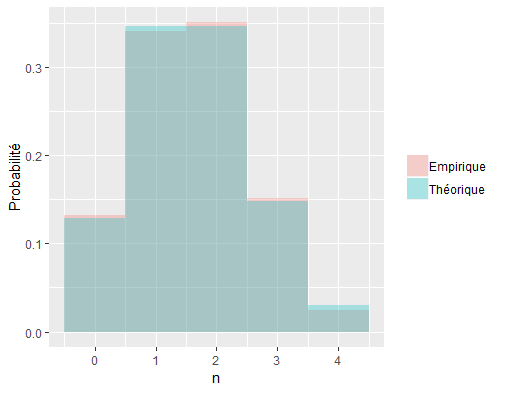
\includegraphics[width=\textwidth]{Graph/geo_log_N.png}
			\caption{Fréquence}
		\end{subfigure}
		%
		\begin{subfigure}[r]{0.5\textwidth}
			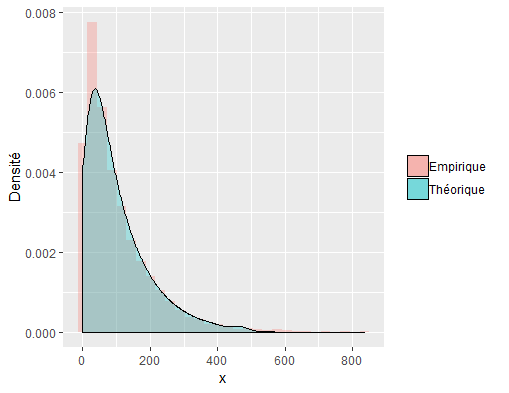
\includegraphics[width=\textwidth]{Graph/geo_log_X.png}
			\caption{Sévérité}
		\end{subfigure}
		\caption{Comparaisons de la distribution marginale des données simulées avec les distributions théoriques pour le scénario \ref{scenario_geo_log}.}
		\label{graph_densite_geo_log}
	\end{figure}
	
	\begin{figure}[H]
		\centering
		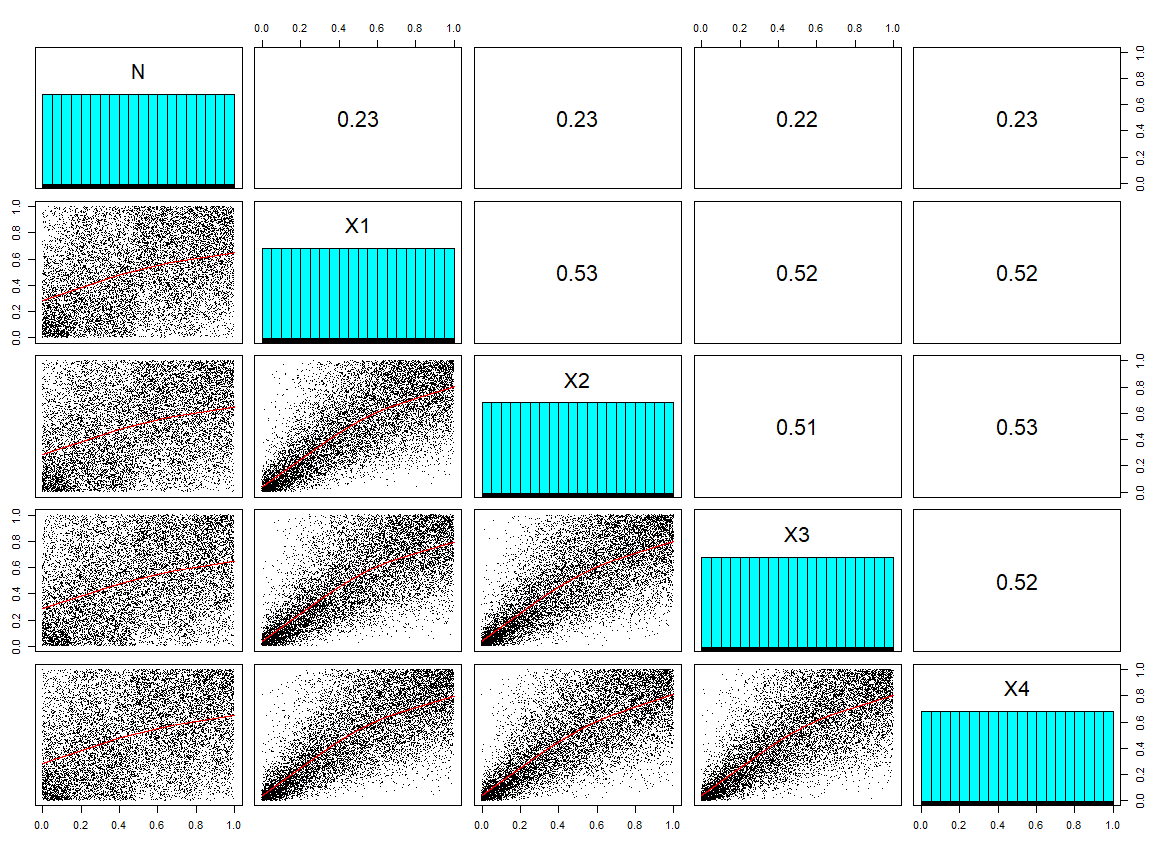
\includegraphics[height=10cm]{Graph/scatterplot_geo_log.png}
		\caption[Nuages de points du scénario \ref{scenario_geo_log}]
		{Nuages de points avec copule archimédienne hiérarchique géométrique-logarithmique($\alpha_0=0.5, \alpha_1 = 0.8$), $N \sim Bin(4, 2/5)$ et $X_i \sim X \sim Exp(1/100)$, pour $i=1,\dots, 4$.:
			En bas de la diagonale se trouve les nuages de points illustrant la corrélation des différentes variables. En haut, on indique les coefficients de corrélation de Spearman. À noter que ce graphique est produit avec la fonction \texttt{R} \texttt{pairs.panels} du module \texttt{psych}. Dans cette dernière, le calcul des coefficients de corrélation sont calculés selon l'hypothèse que les variables sont continues. Cela implique que la première ligne n'est pas valide.}
		\label{graph_scatterplot_geo_log}
	\end{figure}

	Les valeurs de départ de l'optimisation numérique ainsi que les résultats de l'estimation sont présentés dans le tableau \ref{tbl_resultats_geo_log}.
	
	\begin{table}[H]
		\centering
		\begin{tabular}{lrrrr}
			\hline
			& $q$ & $\beta$ & $\alpha_0$ & $\alpha_1$ \\ 
			\hline
			Valeurs de départ & 0.3987 & 0.0101 & 0.5000 & 0.5000 \\ 
			Estimateurs & 0.3990 & 0.0101 & 0.4971 & 0.8712 \\ 
			Vrais paramètres & 0.4000 & 0.0100 & 0.5000 & 0.8000 \\
			\hline
		\end{tabular}
		%
		\begin{tabular}{lr}
			\hline
			&  \\ 
			\hline
			Temps de dérivation & 57.38 \\ 
			Temps d'estimation & 149.72 \\
			\\
			\hline
		\end{tabular}
		\caption[Résultats du scénario \ref{scenario_geo_log}]{Résultats de l'estimation des paramètres avec une copule archimédienne hiérarchique géométrique-logarithmique($\alpha_0=0.5, \alpha_1 = 0.8$), $N \sim Bin(4, 2/5)$ et $X_i \sim X \sim Exp(1/100)$, pour $i=1,\dots,4$, à la suite de 10\,000 simulations.}
		\label{tbl_resultats_geo_log}
	\end{table}



% Scénario 7 : geo-gamma
	\begin{Scenario}\label{scenario_geo_gamma}
		\textbf{Géométrique-Gamma}
	\end{Scenario}
	
	Soit $\Theta_0 \sim Geo(1-\alpha_0)$ avec $E[M] = \frac{1}{1-\alpha_0},\ \mathscr{L}_{\Theta_0} = \frac{1-\alpha_0}{e^t-\alpha_0}$ et $\mathscr{L}^{-1}_{\Theta_0} = \ln\left(\frac{1 - \alpha_0}{u}+\alpha_0\right)$.
	%
	Soit $B_i \sim B \sim gamma(1/\alpha_1,1)$ avec $\mathscr{L}_{B} = (1+t)^{-1/\alpha_1}$ et $\mathscr{L}^{-1}_{B} = u^{-\alpha_1} - 1$. Avec $\alpha_0 = 0.5$, $\alpha_1 = 0.8$, $N\sim Bin(n=5, q=2/5)$ et $X_i \sim X \sim Exp(\beta = 1/100)$, on obtient le sommaire des simulations présenté dans le tableau \ref{tbl_sommaire_geo_gamma} ainsi que les illustrations \ref{graph_densite_geo_gamma} et \ref{graph_scatterplot_geo_gamma}.
	
	\begin{table}[H]
		\centering
		\begin{tabular}{lll}
			\hline
			$N$ &       $X_1$ &       $X_2$        \\ 
			\hline
			  Min.   :0.000   & Min.   :  0.0006   & Min.   :  0.0005    \\ 
			  1st Qu.:1.000   & 1st Qu.: 29.2505   & 1st Qu.: 29.1884    \\ 
			  Median :2.000   & Median : 69.6601   & Median : 70.7418       \\ 
			  Mean   :2.002   & Mean   :100.0527   & Mean   :100.3462       \\ 
			  3rd Qu.:3.000   & 3rd Qu.:138.5964   & 3rd Qu.:138.9114      \\ 
			  Max.   :5.000   & Max.   :908.6793   & Max.   :924.0011   \\ 
			\hline
		\end{tabular}
		%
		\begin{tabular}{lll}
			\hline
			$X_3$ &       $X_4$ &       $X_5$ \\ 
			\hline
			  Min.   :   0.0005   & Min.   :  0.0005   & Min.   :  0.0008   \\ 
			  1st Qu.:  29.2432   & 1st Qu.: 29.1898   & 1st Qu.: 29.4361   \\ 
			  Median :  69.1627   & Median : 70.8558   & Median : 69.3439   \\ 
			  Mean   : 100.4765   & Mean   :101.3061   & Mean   :101.1562   \\ 
			  3rd Qu.: 139.4879   & 3rd Qu.:139.4048   & 3rd Qu.:139.4248   \\ 
			  Max.   :1208.1788   & Max.   :916.6048   & Max.   :846.3202   \\   
			\hline
		\end{tabular}
		\caption[Sommaire des données simulées pour le scénario \ref{scenario_geo_gamma}]{Sommaire de $10\,000$ simulations de $\{N, X_1, \dots, X_5\}$ en supposant que $F_{N,X_1,\dots, X_5}$ est définie avec une copule de archimédienne hiérarchique géométrique-gamma($\alpha_0=0.5, \alpha_1 = 0.8$), $N \sim Bin(5, 2/5)$ et $X_i \sim X \sim Exp(1/100)$, pour $i=1,\dots, 5$.}
		\label{tbl_sommaire_geo_gamma}
	\end{table}
	
	\begin{figure}[H]
		\begin{subfigure}[l]{0.5\textwidth}
			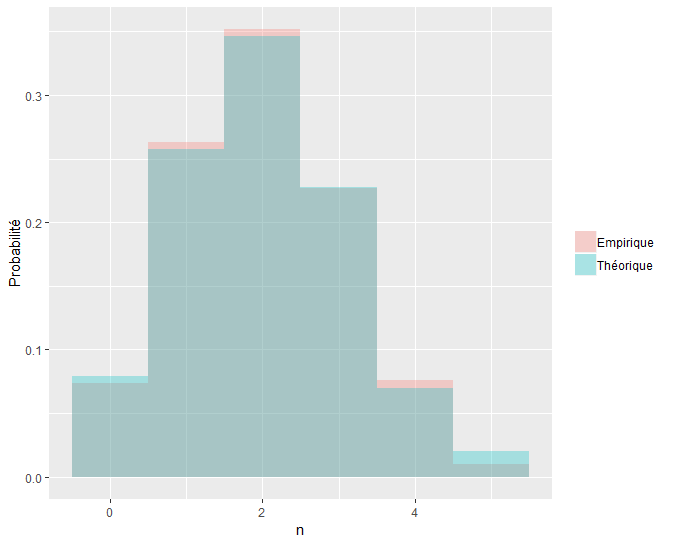
\includegraphics[width=\textwidth]{Graph/geo_gamma_N.png}
			\caption{Fréquence}
		\end{subfigure}
		%
		\begin{subfigure}[r]{0.5\textwidth}
			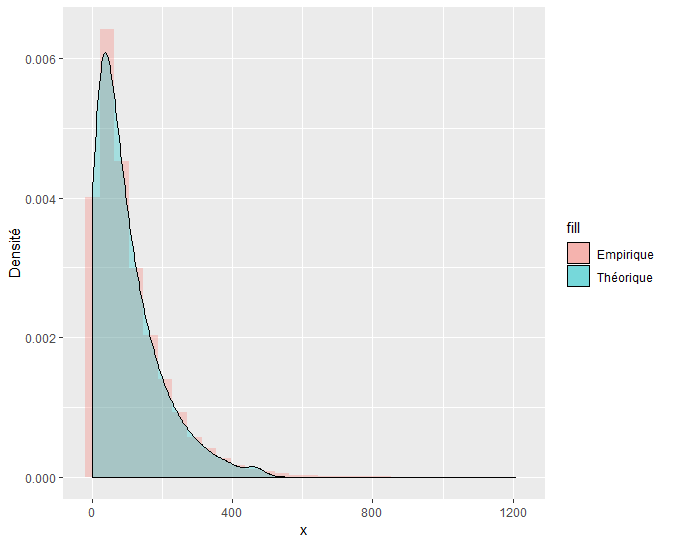
\includegraphics[width=\textwidth]{Graph/geo_gamma_X.png}
			\caption{Sévérité}
		\end{subfigure}
		\caption{Comparaisons de la distribution marginale des données simulées avec les distributions théoriques pour le scénario \ref{scenario_geo_gamma}.}
		\label{graph_densite_geo_gamma}
	\end{figure}
	
	\begin{figure}[H]
		\centering
		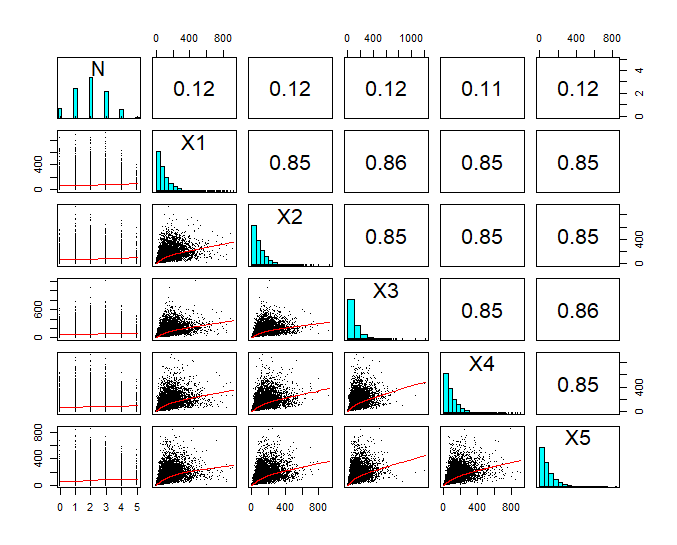
\includegraphics[height=10cm]{Graph/scatterplot_geo_gamma.png}
		\caption[Nuages de points du scénario \ref{scenario_geo_gamma}]
		{Nuages de points avec copule archimédienne hiérarchique géométrique-gamma($\alpha_0=0.5, \alpha_1 = 0.8$), $N \sim Bin(5, 2/5)$ et $X_i \sim X \sim Exp(1/100)$, pour $i=1,\dots, 5$.:
			En bas de la diagonale se trouve les nuages de points illustrant la corrélation des différentes variables. En haut, on indique les coefficients de corrélation de Spearman. À noter que ce graphique est produit avec la fonction \texttt{R} \texttt{pairs.panels} du module \texttt{psych}. Dans cette dernière, le calcul des coefficients de corrélation sont calculés selon l'hypothèse que les variables sont continues. Cela implique que la première ligne n'est pas valide.}
		\label{graph_scatterplot_geo_gamma}
	\end{figure}

	Les valeurs de départ de l'optimisation numérique ainsi que les résultats de l'estimation sont présentés dans le tableau \ref{tbl_resultats_geo_gamma}.
	
	\begin{table}[H]
		\centering
		\begin{tabular}{lrrrr}
			\hline
			& $q$ & $\beta$ & $\alpha_0$ & $\alpha_1$ \\ 
			\hline
			Valeurs de départ & 0.4005 & 0.0095 & 0.5000 & 4.0000 \\ 
			Estimateurs & 0.4019 & 0.0157 & 0.2503 & 6.1103 \\ 
			Vrais paramètres & 0.4000 & 0.0100 & 0.3000 & 5.0000 \\
			\hline
		\end{tabular}
		%
		\begin{tabular}{lr}
			\hline
			&  \\ 
			\hline
			Temps de dérivation & 57.68 \\ 
			Temps d'estimation & 1846.39 \\ 
			\\
			\hline
		\end{tabular}
		\caption[Résultats du scénario \ref{scenario_geo_gamma}]{Résultats de l'estimation des paramètres avec une copule archimédienne hiérarchique géométrique-gamma($\alpha_0=0.5, \alpha_1=0.8$), $N \sim Bin(5, 2/5)$ et $X_i \sim X \sim Exp(1/100)$, pour $i=1,\dots,5$, à la suite de 10\,000 simulations.}
		\label{tbl_resultats_geo_gamma}
	\end{table}



% Scénario 8 : geo-geo
		\begin{Scenario}\label{scenario_geo_geo}
			\textbf{Géométrique-Géométrique}
		\end{Scenario}
		
		Soit $\Theta_0 \sim Geo(1-\alpha_0)$ avec $E[M] = \frac{1}{1-\alpha_0},\ \mathscr{L}_{\Theta_0} = \frac{1-\alpha_0}{e^t-\alpha_0}$ et $\mathscr{L}^{-1}_{\Theta_0} = \ln\left(\frac{1 - \alpha_0}{u}+\alpha_0\right)$.
		%
			Soit $B_i \sim B \sim Geo(1-\alpha_1)$ avec $E[B] = \frac{1}{1-\alpha_1},\ \mathscr{L}_{B} = \frac{1-\alpha_1}{e^t-\alpha_1}$ et $\mathscr{L}^{-1}_{B} = \ln\left(\frac{1 - \alpha_1}{u}+\alpha_1\right)$. Avec $\alpha_0 = 0.5$, $\alpha_1 = 0.3$, $N\sim Bin(n=4, q=2/5)$ et $X_i \sim X \sim Exp(\beta = 1/100)$, on obtient le sommaire des simulations présenté dans le tableau \ref{tbl_sommaire_geo_geo} ainsi que les illustrations \ref{graph_densite_geo_geo} et \ref{graph_scatterplot_geo_geo}.
		
		\begin{table}[H]
			\centering
			\begin{tabular}{lllll}
				\hline
				$N$ &       $X_1$ &       $X_2$    &  $X_3$ &       $X_4$  \\ 
				\hline
				  Min.   :0.000   & Min.   :   0.0087   & Min.   :  0.0062  & Min.   :   0.0068   & Min.   :   0.0003    \\ 
				  1st Qu.:1.000   & 1st Qu.:  29.1523   & 1st Qu.: 28.7089  & 1st Qu.:  28.6573   & 1st Qu.:  27.7252     \\ 
				  Median :2.000   & Median :  70.0952   & Median : 68.7772  & Median :  70.0095   & Median :  67.3220  \\ 
				  Mean   :1.602   & Mean   : 100.5380   & Mean   :100.13362 & Mean   :  99.6027   & Mean   :  99.9894     \\ 
				  3rd Qu.:2.000   & 3rd Qu.: 140.2621   & 3rd Qu.:140.8914  & 3rd Qu.: 139.3071   & 3rd Qu.: 139.6741    \\ 
				  Max.   :4.000   & Max.   :1471.4156   & Max.   :936.3070  & Max.   :1080.3850   & Max.   :1012.0754 \\ 
				\hline
			\end{tabular}
			\caption[Sommaire des données simulées pour le scénario \ref{scenario_geo_geo}]{Sommaire de $10\,000$ simulations de $\{N, X_1, \dots, X_4\}$ en supposant que $F_{N,X_1,\dots, X_4}$ est définie avec une copule de archimédienne hiérarchique géométrique-géométrique($\alpha_0=0.5, \alpha_1 = 0.3$), $N \sim Bin(4, 2/5)$ et $X_i \sim X \sim Exp(1/100)$, pour $i=1,\dots, 4$.}
			\label{tbl_sommaire_geo_geo}
		\end{table}
		
		\begin{figure}[H]
			\begin{subfigure}[l]{0.5\textwidth}
				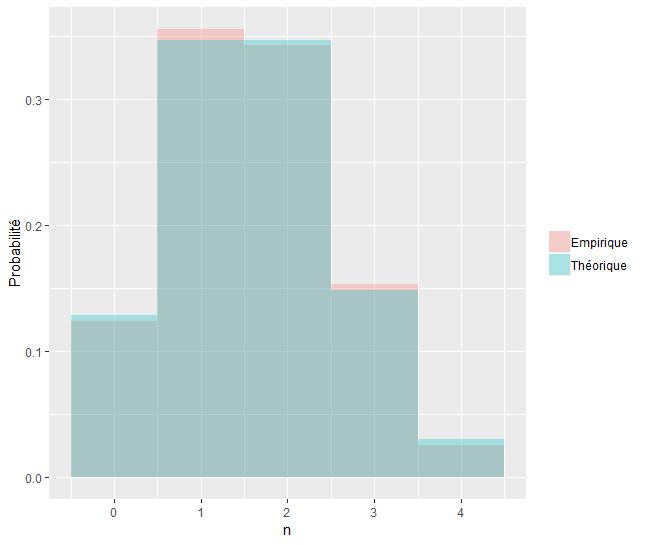
\includegraphics[width=\textwidth]{Graph/geo_geo_N.png}
				\caption{Fréquence}
			\end{subfigure}
			%
			\begin{subfigure}[r]{0.5\textwidth}
				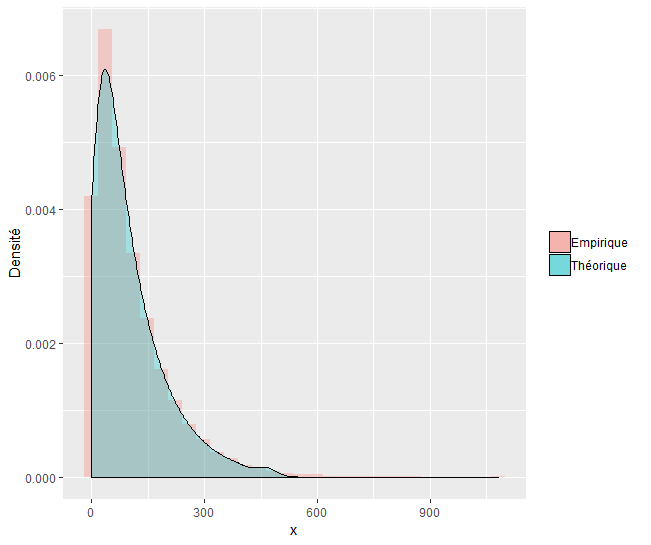
\includegraphics[width=\textwidth]{Graph/geo_geo_X.png}
				\caption{Sévérité}
			\end{subfigure}
			\caption{Comparaisons de la distribution marginale des données simulées avec les distributions théoriques pour le scénario \ref{scenario_geo_geo}.}
			\label{graph_densite_geo_geo}
		\end{figure}
		
		\begin{figure}[H]
			\centering
			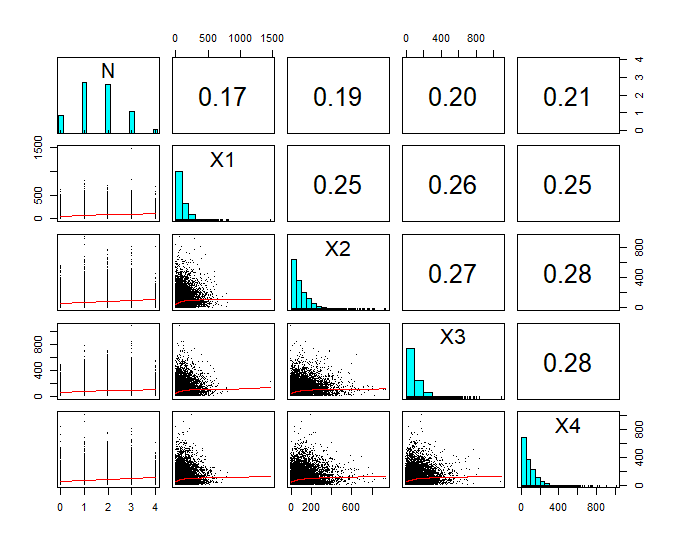
\includegraphics[height=10cm]{Graph/scatterplot_geo_geo.png}
			\caption[Nuages de points du scénario \ref{scenario_geo_geo}]
			{Nuages de points avec copule archimédienne hiérarchique géométrique-géométrique($\alpha_0=0.5, \alpha_1 = 0.3$), $N \sim Bin(4, 2/5)$ et $X_i \sim X \sim Exp(1/100)$, pour $i=1,\dots, 4$.:
				En bas de la diagonale se trouve les nuages de points illustrant la corrélation des différentes variables. En haut, on indique les coefficients de corrélation de Spearman. À noter que ce graphique est produit avec la fonction \texttt{R} \texttt{pairs.panels} du module \texttt{psych}. Dans cette dernière, le calcul des coefficients de corrélation sont calculés selon l'hypothèse que les variables sont continues. Cela implique que la première ligne n'est pas valide.}
			\label{graph_scatterplot_geo_geo}
		\end{figure}
	
		Les valeurs de départ de l'optimisation numérique ainsi que les résultats de l'estimation sont présentés dans le tableau \ref{tbl_resultats_geo_geo}.
		
		\begin{table}[H]
			\centering
			\begin{tabular}{lrrrr}
				\hline
				& $q$ & $\beta$ & $\alpha_0$ & $\alpha_1$ \\ 
				\hline
				Valeurs de départ & 0.4005 & 0.0091 & 0.5000 & 0.5000 \\ 
				Estimateurs & 0.4008 & 0.0099 & 0.5677 & 0.4564 \\ 
				Vrais paramètres & 0.4000 & 0.0100 & 0.5000 & 0.3000 \\ 
				\hline
			\end{tabular}
			%
			\begin{tabular}{lr}
				\hline
				&  \\ 
				\hline
				Temps de dérivation & 15.87 \\ 
				Temps d'estimation & 305.33 \\ 
				\\
				\hline
			\end{tabular}
			\caption[Résultats du scénario \ref{scenario_geo_geo}]{Résultats de l'estimation des paramètres avec une copule archimédienne hiérarchique géométrique-géométrique($\alpha_0=0.5, \alpha_1=0.3$), $N \sim Bin(4, 2/5)$ et $X_i \sim X \sim Exp(1/100)$, pour $i=1,\dots,4$, à la suite de 10\,000 simulations.}
			\label{tbl_resultats_geo_geo}
		\end{table}
	
	
		
	\section{Conclusion}
		Pour conclure, le modèle collectif du risque présenté dans \cite{Itre5} présente un défi dans l'estimation des paramètres par la méthode du maximum de vraisemblance tel que présentée dans la section \ref{sect_Maxlikelyhood} puisque la dérivation en chaîne sur un grand nombre de variables pose un problème de temps de calcul.\\
		
		À cet effet, une solution envisageable pourrait être d'utiliser la vraisemblance par décomposition hiérarchique proposé dans \cite{LikelyhoodEstimation} afin de trouver le paramètre de dépendance entre $N$ et $X_1$, puis de se limiter à un nombre restreint de $X_i$ (disons 5) afin d'estimer le paramètre de dépendance entre les $X_i$. Cependant, avec cette méthode, le fait de travailler avec des variables continues et discrètes cause un problème.
		
		De plus, la difficulté à trouver une valeur de départ adéquate pour $\alpha_{0}$ et $\alpha_{1}$ fait en sorte que les estimateurs de ces paramètres manquent de précision.
	 
		
	\clearpage
	\bibliography{BibRRT_Presentation_2019-05-31.bib}
	\bibliographystyle{apalike}

\end{document}
 